\usetikzlibrary{arrows.meta,positioning,shapes.geometric,shapes.misc,calc,fit,backgrounds}
\usetikzlibrary{decorations.pathmorphing,decorations.markings,automata,mindmap,trees,shadows}
\usetikzlibrary{lindenmayersystems}
\usepgfplotslibrary{fillbetween,polar}

\section{K1: lo que sabe pintar este motor}

Este documento recorre las capacidades de N-LTX con ejemplos reales. Todo lo que hay aquí nace de una sola fuente LaTeX: Rust la compone y la GPU la pinta en una única superficie, de modo que el texto, las fórmulas, las figuras y las animaciones comparten documento, desplazamiento y zoom.

\begin{itemize}
\item \textbf{Texto}: títulos, párrafos, listas, tablas, citas, código y notas.
\item \textbf{Matemáticas}: álgebra, cálculo, álgebra lineal, probabilidad, lógica, geometría y gráficas.
\item \textbf{Física}: mecánica, electromagnetismo, termodinámica, relatividad, cuántica, óptica y unidades.
\item \textbf{Química}: reacciones, moléculas, esquemas, equilibrio y tabla periódica.
\item \textbf{Diagramas}: flujo, estados, árboles, grafos, redes, secuencias y mapas conceptuales.
\item \textbf{Electrónica}: circuitos analógicos y digitales.
\item \textbf{Animaciones}: mecanismos, ondas, campos, partículas, moléculas y algoritmos en movimiento.
\end{itemize}

\section{Texto}

\subsection{Párrafos y estilos}

Un párrafo fluye al ancho de la columna y se recompone al cambiar el tamaño de la ventana. Dentro de él conviven la \textbf{negrita}, la \emph{cursiva}, la \textbf{\emph{negrita cursiva}}, el \texttt{texto monoespaciado}, el \underline{subrayado} y el \textcolor{blue}{color}, además de los signos del español: ¿qué?, ¡sí!, «comillas», año, pingüino, corazón.

Las fórmulas en línea se alinean con el texto, tanto las bajas como $E=mc^2$ como las altas: $\frac{a+b}{c+d}$, $\sqrt{1+\sqrt{x}}$ o $\sum_{k=1}^{n}k$. También entran las unidades, como \SI{9.81}{m/s^2}, y la química, como \ce{H2SO4}.\footnote{Las notas al pie se recogen al final del documento.} Las citas se señalan así \cite{knuth} y los enlaces se subrayan: \href{https://ctan.org}{la red de archivos de TeX}.

\subsection{Listas}

Las listas se anidan y admiten fórmulas:

\begin{enumerate}
\item Plantea el problema: $f(x)=0$.
\item Elige un método:
  \begin{itemize}
  \item bisección, si $f$ es continua y cambia de signo;
  \item Newton, si conoces $f'$: $x_{n+1}=x_n-\frac{f(x_n)}{f'(x_n)}$;
  \item secante, si no la conoces.
  \end{itemize}
\item Comprueba el resultado.
\end{enumerate}

\begin{description}
\item[Vulkan] la interfaz gráfica de bajo nivel que usa el pintor.
\item[Teselado] convertir curvas en triángulos para la GPU.
\item[Atlas] una textura que guarda los glifos ya rasterizados.
\end{description}

\subsection{Tablas}

Una tabla es una rejilla más un estilo. Sin decir nada, usa el tema: la cabecera reparte su paleta por las columnas, las filas van separadas por un hueco y cada columna toma el ancho que necesita.

\begin{tabular}{lccr}
Planeta & Órbita (ua) & Lunas & Periodo (días) \\
Mercurio & $0{,}39$ & 0 & 88 \\
Venus & $0{,}72$ & 0 & 225 \\
Tierra & $1{,}00$ & 1 & 365 \\
Marte & $1{,}52$ & 2 & 687 \\
Júpiter & $5{,}20$ & 95 & 4333 \\
\end{tabular}

Los colores se cambian desde la fuente, con una lista repartida por las columnas, y el texto busca solo el contraste:

\begin{tabular}[cabecera={orange!80!black,red!70!black,violet},filas={orange!8,white}]{lcc}
Magnitud & Símbolo & Unidad \\
Fuerza & $F$ & \si{N} \\
Energía & $E$ & \si{J} \\
Potencia & $P$ & \si{W} \\
Presión & $p$ & \si{Pa} \\
\end{tabular}

Un estilo con nombre sirve para todas las tablas que lo pidan, y otro puede heredar de él:

\estilotabla{sobria}{cabecera=gray!25,filas=no,reglas=gray!40,separacion=0,texto cabecera=black}
\estilotabla{sobria azul}{estilo=sobria,cabecera=blue!15}

\begin{tabular}[estilo=sobria]{lrr}
Ensayo & Tiempo (ms) & Error (\%) \\
Primero & 12,4 & 0,8 \\
Segundo & 11,9 & 0,6 \\
Tercero & 12,1 & 0,7 \\
\end{tabular}

\begin{tabular}[estilo=sobria azul]{lrr}
Ensayo & Tiempo (ms) & Error (\%) \\
Primero & 12,4 & 0,8 \\
Segundo & 11,9 & 0,6 \\
\end{tabular}

Las celdas pueden ocupar varias columnas o filas, y cada fila o celda puede llevar su propio color:

\begin{tabular}{lcccc}
\multirow{2}{*}{\textbf{Ciudad}} & \multicolumn{2}{c}{Invierno} & \multicolumn{2}{c}{Verano} \\
 & Mín. & Máx. & Mín. & Máx. \\
Madrid & 3 & 10 & 19 & 33 \\
\rowcolor{yellow!25} Sevilla & 6 & 16 & 21 & 36 \\
Bilbao & 6 & 13 & \cellcolor{green!20}16 & \cellcolor{green!20}25 \\
\end{tabular}

Y una celda lleva lo mismo que un párrafo: fórmulas, química y varias líneas de distinto tamaño.

\begin{tabular}[cabecera={teal,blue!70!black},columnas=iguales]{ccc}
Ecuación & Reacción & Elemento \\
$E=mc^2$ & \ce{2H2 + O2 -> 2H2O} & \makecell{\tiny 79\\\textbf{Au}\\\tiny Oro} \\
$\int_0^1 x^2\,dx=\frac{1}{3}$ & \ce{CH4 + 2O2 -> CO2 + 2H2O} & \makecell{\tiny 26\\\textbf{Fe}\\\tiny Hierro} \\
\end{tabular}

\subsection{Citas y código}

\begin{quote}
Las matemáticas son el arte de dar el mismo nombre a cosas distintas.
\end{quote}

Un bloque de código se ve como un editor: con su pestaña, sus líneas numeradas, guías de sangría, una tipografía hecha para leer código y los colores de su lenguaje. El nombre de la pestaña se pide con \texttt{title=}, y \texttt{guias=no} quita las guías.

\begin{lstlisting}[language=Rust,title=fibonacci.rs]
/// El n-ésimo número de Fibonacci.
fn fibonacci(n: u32) -> u64 {
    let (mut a, mut b) = (0, 1);
    for _ in 0..n {
        (a, b) = (b, a + b);
    }
    a
}
\end{lstlisting}

\begin{lstlisting}[language=Python,title=particula.py]
from dataclasses import dataclass

@dataclass
class Particula:
    masa: float = 1.0  # en kilogramos

    def energia(self, v: float) -> float:
        """Energía cinética."""
        return 0.5 * self.masa * v ** 2
\end{lstlisting}

\begin{lstlisting}[language=C++,title=suma.hpp]
#include <vector>

template <typename T>
T suma(const std::vector<T>& v) {
    T total{};
    for (const auto& x : v) total += x;
    return total;
}
\end{lstlisting}

Si no hay título, la pestaña dice el lenguaje. Una línea demasiado larga para la columna se parte, con un solo número, como en un editor:

\begin{lstlisting}[language=Bash]
# Cuenta las líneas de cada archivo de Rust
for f in src/*.rs; do
    echo "$f: $(wc -l < "$f") líneas, última modificación $(date -r "$f" +%Y-%m-%d), tamaño $(du -h "$f" | cut -f1)"
done
\end{lstlisting}

\begin{lstlisting}[language=JSON]
{
  "elemento": "Sodio",
  "numero": 11,
  "estable": true
}
\end{lstlisting}

\begin{lstlisting}[language=LaTeX]
\begin{equation}
  e^{i\pi} + 1 = 0
\end{equation}
\end{lstlisting}

La numeración puede empezar donde haga falta, para citar un trozo de un archivo:

\begin{lstlisting}[language=Rust,title=main.rs,firstnumber=128]
fn main() {
    let total: u64 = (1..=10).map(fibonacci).sum();
    println!("{total}");
}
\end{lstlisting}

El tema cambia el editor entero: la sintaxis, el fondo y los números. Hay una treintena, y \texttt{estilocodigo} cambia el de todos los bloques.

\begin{lstlisting}[language=Python,title=tema Dracula,tema=Dracula]
def cuadrado(x):
    return x * x  # en cualquier tema
\end{lstlisting}

\begin{lstlisting}[language=Python,title=tema Nord,tema=Nord]
def cuadrado(x):
    return x * x  # en cualquier tema
\end{lstlisting}

\begin{lstlisting}[language=Python,title=tema OneHalfLight,tema=OneHalfLight]
def cuadrado(x):
    return x * x  # en cualquier tema
\end{lstlisting}

Sin lenguaje, el bloque se queda en texto plano, y sin números si se pide con \texttt{numbers=none}:

\begin{lstlisting}[numbers=none]
Entrada: 5 2 8 1
Salida:  1 2 5 8
\end{lstlisting}

\section{Matemáticas}

\subsection{Álgebra}

La fórmula general de segundo grado, el binomio de Newton y la identidad de Euler:

\[ x=\frac{-b\pm\sqrt{b^2-4ac}}{2a} \]

\[ (a+b)^n=\sum_{k=0}^{n}\binom{n}{k}a^{n-k}b^k \]

\[ e^{i\pi}+1=0 \]

Fracciones continuas, raíces anidadas y productos notables:

\[ \varphi=1+\cfrac{1}{1+\cfrac{1}{1+\cfrac{1}{1+\cdots}}}=\frac{1+\sqrt{5}}{2} \]

\[ \sqrt{2+\sqrt{2+\sqrt{2+\sqrt{2}}}}=2\cos\frac{\pi}{32} \]

\begin{align*}
(a+b)(a-b) &= a^2-b^2 \\
(a+b)^3 &= a^3+3a^2b+3ab^2+b^3 \\
a^3-b^3 &= (a-b)(a^2+ab+b^2)
\end{align*}

Varias ecuaciones centradas, y una sola demasiado larga para una línea:

\begin{gather*}
\sin^2 x+\cos^2 x=1 \\
\sin(a+b)=\sin a\cos b+\cos a\sin b \\
e^{ix}=\cos x+i\sin x
\end{gather*}

\begin{multline*}
(x+y+z)^3=x^3+y^3+z^3+3x^2y+3x^2z \\
+3y^2x+3y^2z+3z^2x+3z^2y+6xyz
\end{multline*}

Funciones definidas por trozos, llaves con texto y colores:

\[ |x|=\begin{cases} x & \text{si } x\ge 0 \\ -x & \text{si } x<0 \end{cases} \]

\[ \overbrace{1+2+\cdots+n}^{n\ \text{términos}}=\frac{n(n+1)}{2} \qquad \underbrace{a+a+\cdots+a}_{k\ \text{veces}}=ka \]

\[ \textcolor{red}{\boldsymbol{\alpha}}+\textcolor{blue}{\boldsymbol{\beta}}=\textcolor{violet}{\boldsymbol{\gamma}} \]

\subsection{Cálculo}

Límites, derivadas e integrales:

\[ \lim_{x\to 0}\frac{\sin x}{x}=1 \qquad \lim_{n\to\infty}\left(1+\frac{1}{n}\right)^n=e \]

\[ f'(x)=\lim_{h\to 0}\frac{f(x+h)-f(x)}{h} \]

\[ \int_{-\infty}^{\infty}e^{-x^2}\,dx=\sqrt{\pi} \qquad \int_{0}^{\infty}\frac{\sin x}{x}\,dx=\frac{\pi}{2} \]

\[ \frac{d}{dx}\int_{a}^{x}f(t)\,dt=f(x) \]

Series de Taylor, de Fourier y el problema de Basilea:

\[ e^x=\sum_{n=0}^{\infty}\frac{x^n}{n!}=1+x+\frac{x^2}{2!}+\frac{x^3}{3!}+\cdots \]

\[ f(x)=\frac{4}{\pi}\sum_{k=0}^{\infty}\frac{\sin\big((2k+1)x\big)}{2k+1} \]

\[ \zeta(2)=\sum_{n=1}^{\infty}\frac{1}{n^2}=\frac{\pi^2}{6} \]

Cálculo vectorial y transformadas:

\[ \oint_{\partial S}\vb{F}\cdot d\vb{l}=\iint_{S}\left(\nabla\times\vb{F}\right)\cdot d\vb{S} \]

\[ \oiint_{\partial V}\vb{F}\cdot d\vb{S}=\iiint_{V}\nabla\cdot\vb{F}\,dV \]

\[ \hat{f}(\xi)=\int_{-\infty}^{\infty}f(x)\,e^{-2\pi i x\xi}\,dx \]

\subsection{Álgebra lineal}

\[ \begin{pmatrix} a & b \\ c & d \end{pmatrix}^{-1}=\frac{1}{ad-bc}\begin{pmatrix} d & -b \\ -c & a \end{pmatrix} \]

\[ \det\begin{bmatrix} a & b & c \\ d & e & f \\ g & h & i \end{bmatrix}=aei+bfg+cdh-ceg-bdi-afh \]

\[ \begin{vmatrix} 1 & x_1 & x_1^2 \\ 1 & x_2 & x_2^2 \\ 1 & x_3 & x_3^2 \end{vmatrix}=\prod_{i<j}(x_j-x_i) \]

\[ A\vb{v}=\lambda\vb{v} \qquad A=U\Sigma V^{\mathsf{T}} \qquad \operatorname{tr}(AB)=\operatorname{tr}(BA) \]

\[ \left[\begin{array}{ccc|c} 1 & 2 & 3 & 6 \\ 0 & 1 & 4 & 5 \\ 0 & 0 & 1 & 1 \end{array}\right] \]

\[ \begin{pmatrix} a_{11} & a_{12} & \cdots & a_{1n} \\ a_{21} & a_{22} & \cdots & a_{2n} \\ \vdots & \vdots & \ddots & \vdots \\ a_{m1} & a_{m2} & \cdots & a_{mn} \end{pmatrix} \]

\subsection{Probabilidad y estadística}

\[ f(x)=\frac{1}{\sigma\sqrt{2\pi}}\exp\left(-\frac{(x-\mu)^2}{2\sigma^2}\right) \]

\[ P(A\mid B)=\frac{P(B\mid A)\,P(A)}{P(B)} \]

\[ \mathbb{E}[X]=\sum_i x_i\,p_i \qquad \operatorname{Var}(X)=\mathbb{E}\big[(X-\mu)^2\big] \]

\[ H(X)=-\sum_{i}p_i\log_2 p_i \]

\[ P(X=k)=\binom{n}{k}p^k(1-p)^{n-k} \qquad P(X=k)=\frac{\lambda^k e^{-\lambda}}{k!} \]

\subsection{Números, conjuntos y lógica}

\[ \zeta(s)=\sum_{n=1}^{\infty}\frac{1}{n^s}=\prod_{p\ \text{primo}}\frac{1}{1-p^{-s}} \]

\[ a^{p-1}\equiv 1 \pmod{p} \qquad n!\sim\sqrt{2\pi n}\left(\frac{n}{e}\right)^n \]

\[ \forall\varepsilon>0\ \exists\delta>0:\ |x-a|<\delta\implies|f(x)-f(a)|<\varepsilon \]

\[ \mathbb{N}\subset\mathbb{Z}\subset\mathbb{Q}\subset\mathbb{R}\subset\mathbb{C} \qquad A\cap(B\cup C)=(A\cap B)\cup(A\cap C) \]

\[ \neg(p\land q)\iff\neg p\lor\neg q \]

\subsection{Diagramas conmutativos}

\[ \begin{tikzcd} A \arrow[r,"f"] \arrow[d,"g"'] & B \arrow[d,"h"] \\ C \arrow[r,"k"'] & D \end{tikzcd} \]

\[ \begin{tikzcd} 0 \arrow[r] & A \arrow[r,"\iota"] & B \arrow[r,"\pi"] & C \arrow[r] & 0 \end{tikzcd} \]

\subsection{Geometría}

\begin{figure}
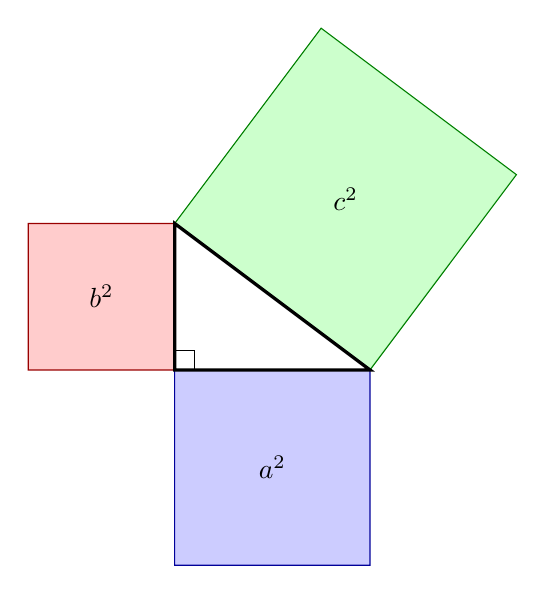
\begin{tikzpicture}[scale=0.62]
  \coordinate (A) at (0,0);
  \coordinate (B) at (4,0);
  \coordinate (C) at (0,3);
  \fill[blue!20,draw=blue!60!black] (A) -- (B) -- (4,-4) -- (0,-4) -- cycle;
  \fill[red!20,draw=red!60!black] (A) -- (C) -- (-3,3) -- (-3,0) -- cycle;
  \fill[green!20,draw=green!50!black] (B) -- (7,4) -- (3,7) -- (C) -- cycle;
  \draw[very thick] (A) -- (B) -- (C) -- cycle;
  \draw (0.4,0) -- (0.4,0.4) -- (0,0.4);
  \node at (2,-2) {$a^2$};
  \node at (-1.5,1.5) {$b^2$};
  \node at (3.5,3.5) {$c^2$};
  \node[below] at (2,0.05) {};
\end{tikzpicture}
\caption{Teorema de Pitágoras: el área sobre la hipotenusa es la suma de las otras dos.}
\end{figure}

\begin{figure}
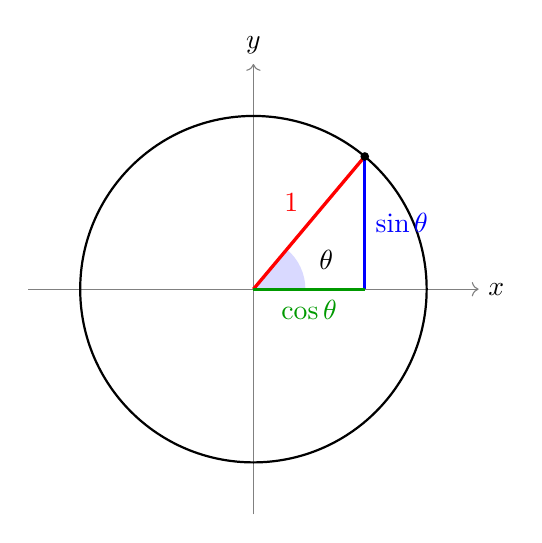
\begin{tikzpicture}[scale=2.2]
  \draw[->,gray] (-1.3,0) -- (1.3,0) node[right,black] {$x$};
  \draw[->,gray] (0,-1.3) -- (0,1.3) node[above,black] {$y$};
  \draw[thick] (0,0) circle (1);
  \fill[blue!15] (0,0) -- (0.3,0) arc (0:50:0.3) -- cycle;
  \draw[very thick,red] (0,0) -- (50:1) node[midway,above left] {$1$};
  \draw[very thick,blue] ({cos(50)},0) -- (50:1) node[midway,right] {$\sin\theta$};
  \draw[very thick,green!60!black] (0,0) -- ({cos(50)},0) node[midway,below] {$\cos\theta$};
  \node at (0.42,0.17) {$\theta$};
  \fill (50:1) circle (0.025);
\end{tikzpicture}
\caption{Circunferencia unidad: $\sin^2\theta+\cos^2\theta=1$.}
\end{figure}

\begin{figure}
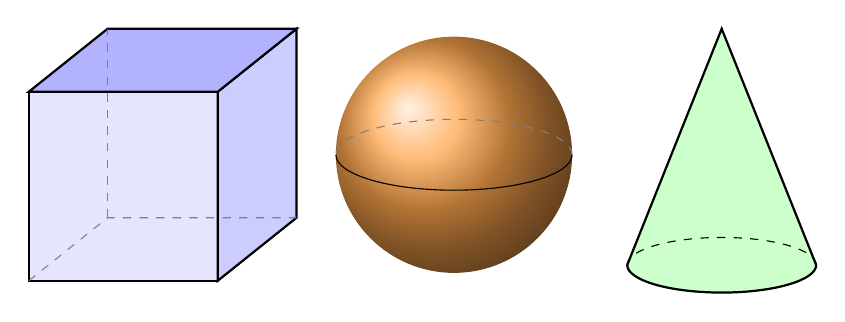
\begin{tikzpicture}
  \draw[thick,fill=blue!10] (0,0) rectangle (2.4,2.4);
  \draw[thick,fill=blue!20] (2.4,0) -- (3.4,0.8) -- (3.4,3.2) -- (2.4,2.4) -- cycle;
  \draw[thick,fill=blue!30] (0,2.4) -- (1,3.2) -- (3.4,3.2) -- (2.4,2.4) -- cycle;
  \draw[dashed,gray] (0,0) -- (1,0.8) -- (3.4,0.8);
  \draw[dashed,gray] (1,0.8) -- (1,3.2);
  \begin{scope}[xshift=5.4cm,yshift=1.6cm]
    \shade[ball color=orange!70] (0,0) circle (1.5);
    \draw[dashed,gray] (1.5,0) arc (0:180:1.5 and 0.45);
    \draw (-1.5,0) arc (180:360:1.5 and 0.45);
  \end{scope}
  \begin{scope}[xshift=8.8cm,yshift=0.2cm]
    \fill[green!20] (-1.2,0) arc (180:360:1.2 and 0.35) -- (0,3) -- cycle;
    \draw[thick] (-1.2,0) -- (0,3) -- (1.2,0);
    \draw[thick] (-1.2,0) arc (180:360:1.2 and 0.35);
    \draw[dashed] (1.2,0) arc (0:180:1.2 and 0.35);
  \end{scope}
\end{tikzpicture}
\caption{Cuerpos en perspectiva: un cubo, una esfera con sombreado y un cono.}
\end{figure}

\subsection{Gráficas de funciones}

\begin{figure}
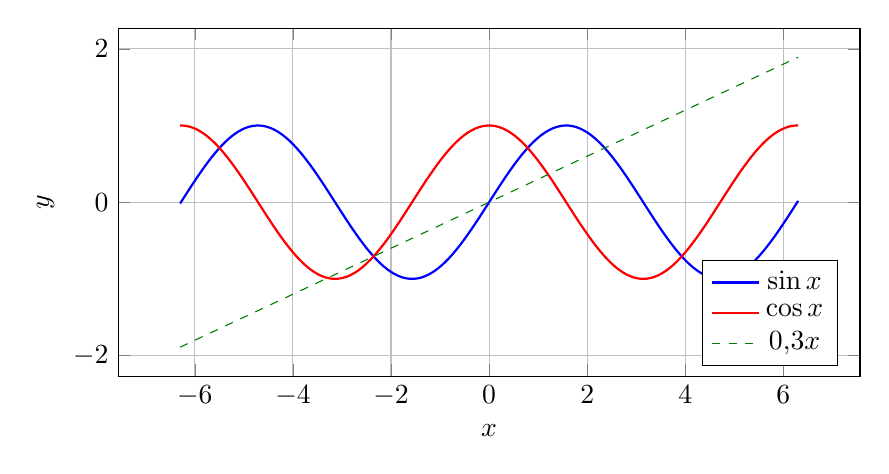
\begin{tikzpicture}
  \begin{axis}[xlabel=$x$,ylabel=$y$,domain=-6.3:6.3,samples=160,width=11cm,height=6cm,grid=major,legend pos=south east]
    \addplot[blue,thick] {sin(deg(x))};
    \addplot[red,thick] {cos(deg(x))};
    \addplot[green!50!black,dashed] {0.3*x};
    \legend{$\sin x$,$\cos x$,$0{,}3x$}
  \end{axis}
\end{tikzpicture}
\caption{Varias funciones, con cuadrícula y leyenda.}
\end{figure}

\begin{figure}
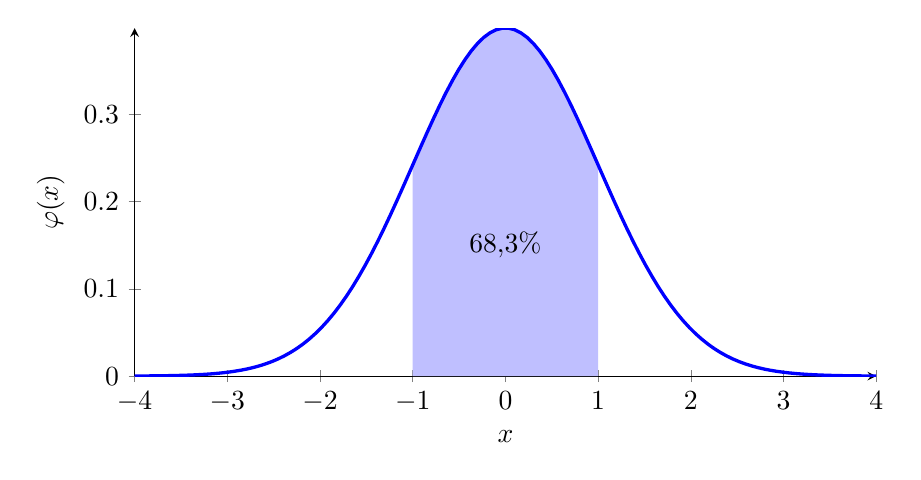
\begin{tikzpicture}
  \begin{axis}[domain=-4:4,samples=120,width=11cm,height=6cm,xlabel=$x$,ylabel=$\varphi(x)$,ymin=0,axis lines=left]
    \addplot[name path=f,blue,very thick] {exp(-x^2/2)/sqrt(2*pi)};
    \path[name path=eje] (axis cs:-4,0) -- (axis cs:4,0);
    \addplot[blue!25] fill between[of=f and eje,soft clip={domain=-1:1}];
    \node at (axis cs:0,0.15) {$68{,}3\%$};
  \end{axis}
\end{tikzpicture}
\caption{Distribución normal: el área a menos de una desviación típica.}
\end{figure}

\begin{figure}
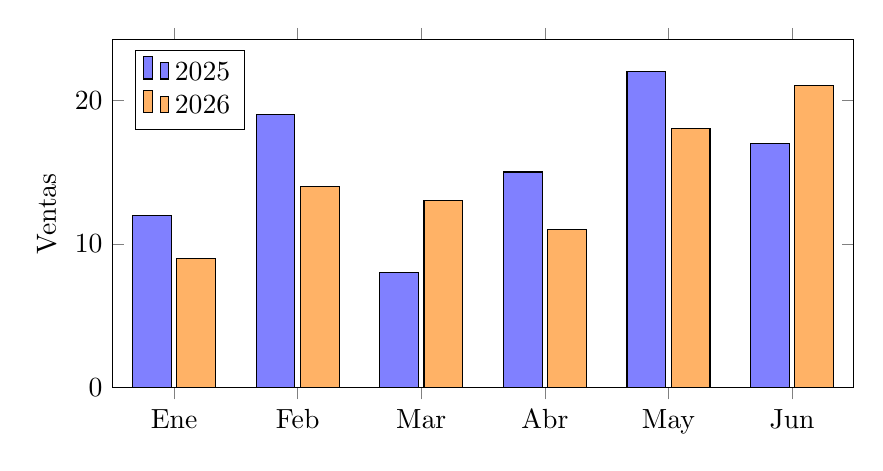
\begin{tikzpicture}
  \begin{axis}[ybar,bar width=14pt,width=11cm,height=6cm,symbolic x coords={Ene,Feb,Mar,Abr,May,Jun},xtick=data,ylabel=Ventas,ymin=0,legend pos=north west]
    \addplot[fill=blue!50] coordinates {(Ene,12) (Feb,19) (Mar,8) (Abr,15) (May,22) (Jun,17)};
    \addplot[fill=orange!60] coordinates {(Ene,9) (Feb,14) (Mar,13) (Abr,11) (May,18) (Jun,21)};
    \legend{2025,2026}
  \end{axis}
\end{tikzpicture}
\caption{Barras agrupadas por categorías.}
\end{figure}

\begin{figure}
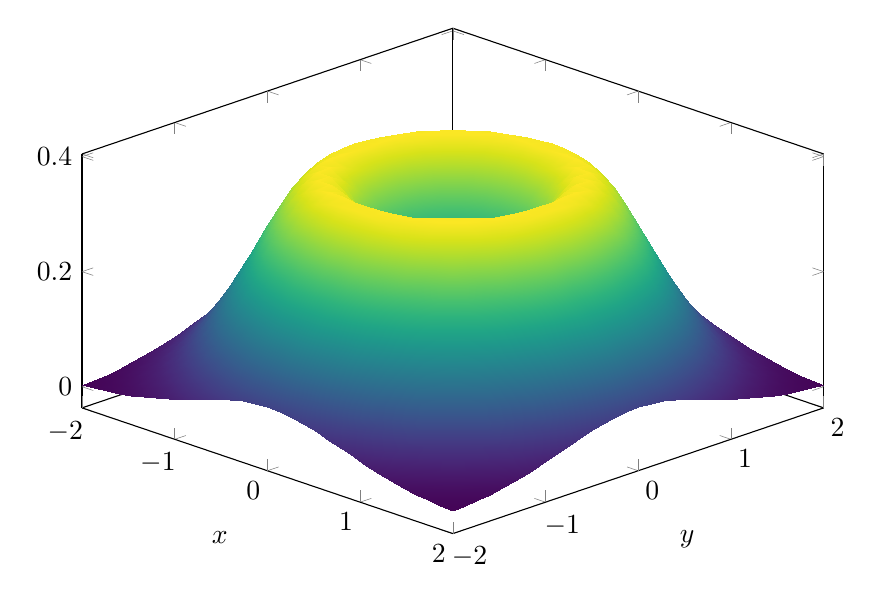
\begin{tikzpicture}
  \begin{axis}[view={45}{35},width=11cm,height=8cm,xlabel=$x$,ylabel=$y$,colormap/viridis,domain=-2:2,y domain=-2:2,samples=31]
    \addplot3[surf,shader=interp] {exp(-x^2-y^2)*(x^2+y^2)};
  \end{axis}
\end{tikzpicture}
\caption{Superficie en tres dimensiones con mapa de color.}
\end{figure}

\begin{figure}
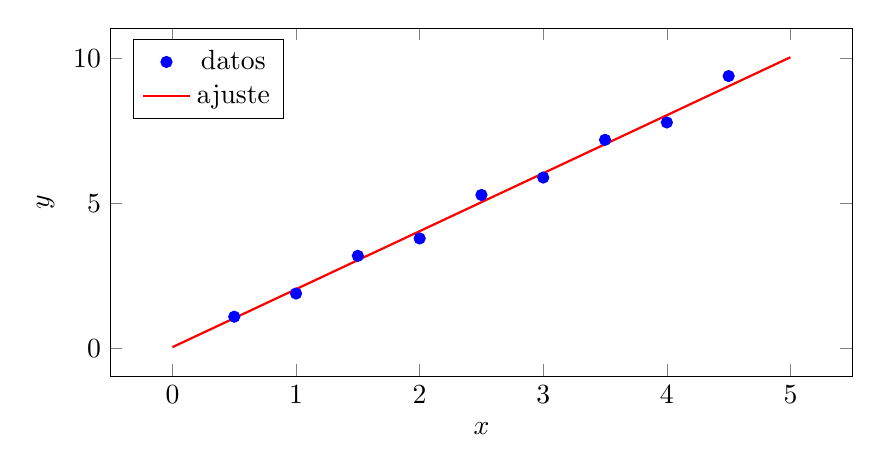
\begin{tikzpicture}
  \begin{axis}[xlabel=$x$,ylabel=$y$,width=11cm,height=6cm,legend pos=north west]
    \addplot[blue,mark=*,only marks] coordinates {(0.5,1.1) (1,1.9) (1.5,3.2) (2,3.8) (2.5,5.3) (3,5.9) (3.5,7.2) (4,7.8) (4.5,9.4)};
    \addplot[red,no marks,thick,domain=0:5] {2*x+0.05};
    \legend{datos,ajuste}
  \end{axis}
\end{tikzpicture}
\caption{Nube de puntos con recta de ajuste.}
\end{figure}

\begin{figure}
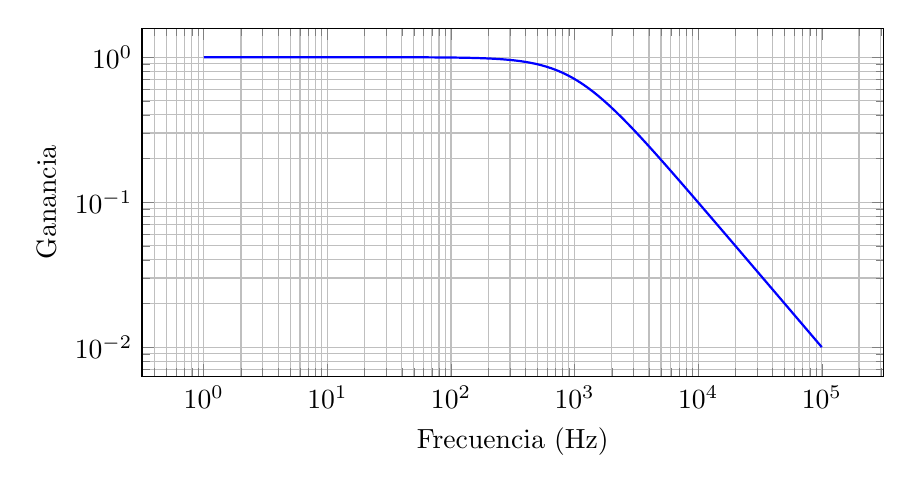
\begin{tikzpicture}
  \begin{axis}[xmode=log,ymode=log,xlabel=Frecuencia (\si{Hz}),ylabel=Ganancia,width=11cm,height=6cm,grid=both]
    \addplot[blue,thick,domain=1:100000,samples=120] {1/sqrt(1+(x/1000)^2)};
  \end{axis}
\end{tikzpicture}
\caption{Ejes logarítmicos: filtro paso bajo de primer orden.}
\end{figure}

\begin{figure}
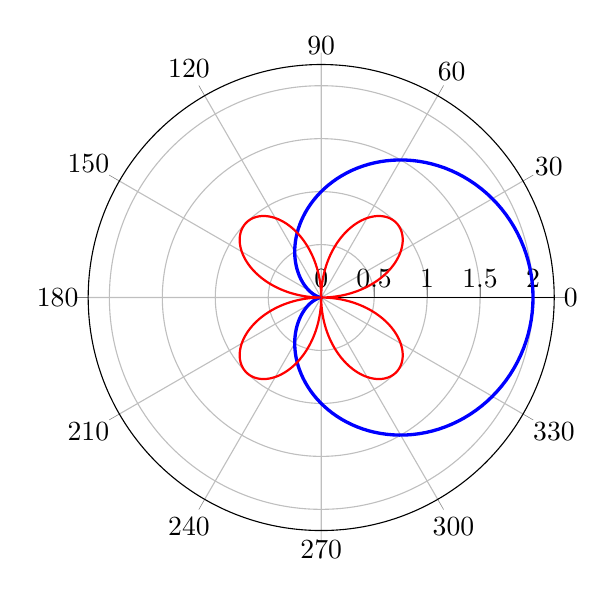
\begin{tikzpicture}
  \begin{polaraxis}[width=7.5cm,height=7.5cm]
    \addplot[blue,very thick,domain=0:360,samples=180] {1+cos(x)};
    \addplot[red,thick,domain=0:360,samples=360] {abs(sin(2*x))};
  \end{polaraxis}
\end{tikzpicture}
\caption{Coordenadas polares: una cardioide y una rosa de cuatro pétalos.}
\end{figure}

\begin{figure}
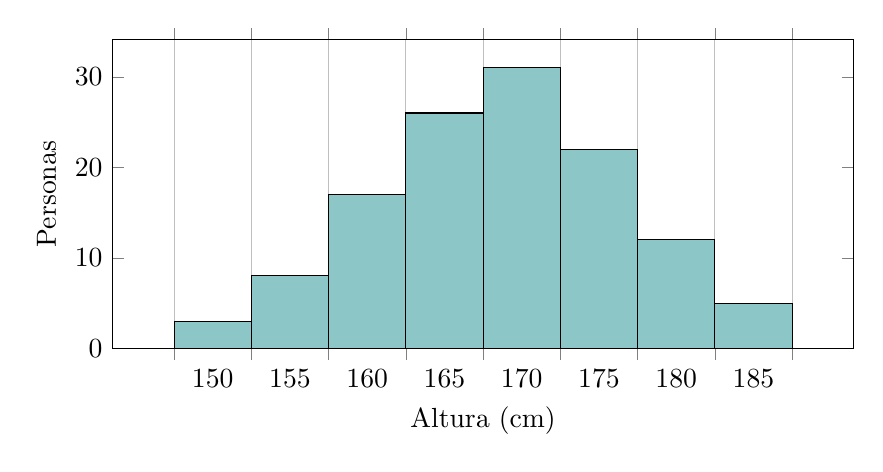
\begin{tikzpicture}
  \begin{axis}[ybar interval,width=11cm,height=5.5cm,ymin=0,xlabel=Altura (\si{cm}),ylabel=Personas,xtick=data]
    \addplot[fill=teal!45] coordinates {(150,3) (155,8) (160,17) (165,26) (170,31) (175,22) (180,12) (185,5) (190,0)};
  \end{axis}
\end{tikzpicture}
\caption{Histograma.}
\end{figure}

\begin{figure}
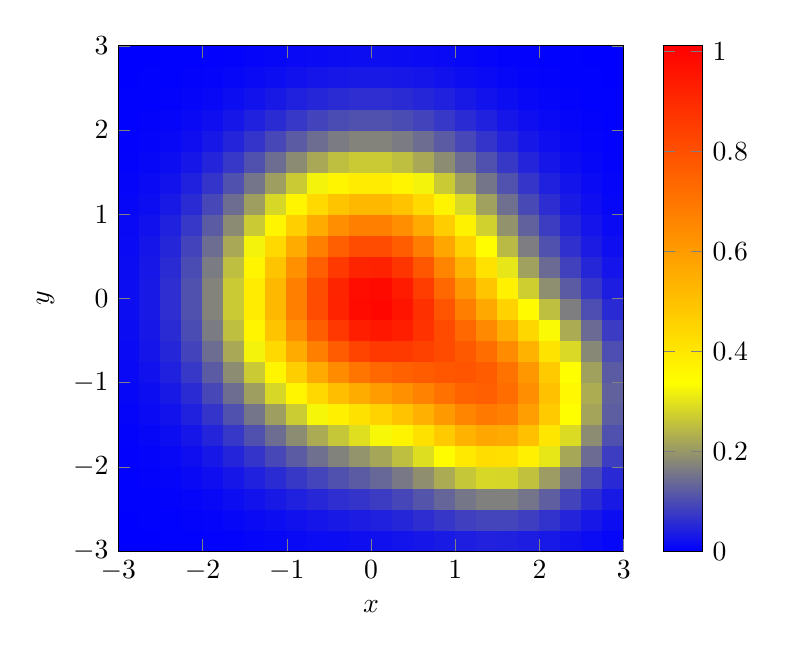
\begin{tikzpicture}
  \begin{axis}[view={0}{90},width=8cm,height=8cm,colorbar,colormap/hot,domain=-3:3,y domain=-3:3,samples=25,xlabel=$x$,ylabel=$y$]
    \addplot3[surf,shader=flat] {exp(-x^2/2-y^2/2)+0.6*exp(-(x-1.6)^2-(y+1.2)^2)};
  \end{axis}
\end{tikzpicture}
\caption{Mapa de calor con barra de color.}
\end{figure}

\section{Física}

\subsection{Mecánica}

La segunda ley de Newton, las ecuaciones de Euler-Lagrange y las de Hamilton:

\[ \vb{F}=m\vb{a}=\dv{\vb{p}}{t} \]

\[ \dv{t}\pdv{L}{\dot{q}_i}-\pdv{L}{q_i}=0 \]

\[ \dot{q}_i=\pdv{H}{p_i} \qquad \dot{p}_i=-\pdv{H}{q_i} \]

La gravitación universal, la tercera ley de Kepler y el oscilador armónico:

\[ F=G\frac{m_1 m_2}{r^2} \qquad T^2=\frac{4\pi^2}{GM}a^3 \]

\[ \dv[2]{x}{t}+2\gamma\dv{x}{t}+\omega_0^2 x=0 \]

\begin{figure}
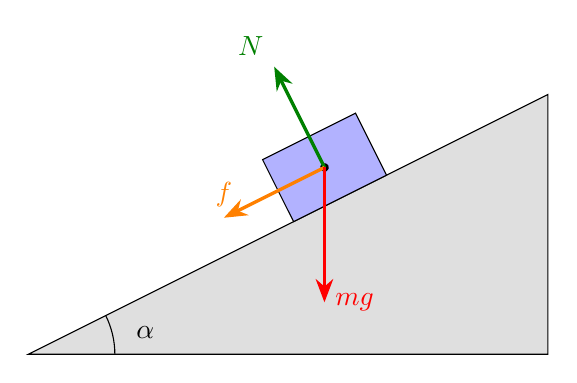
\begin{tikzpicture}[scale=1.1]
  \fill[gray!25,draw=black] (0,0) -- (6,0) -- (6,3) -- cycle;
  \draw (1,0) arc (0:26.57:1);
  \node at (1.35,0.25) {$\alpha$};
  \begin{scope}[shift={(3.6,1.8)},rotate=26.57]
    \fill[blue!30,draw=black] (-0.6,0) rectangle (0.6,0.8);
    \fill (0,0.4) circle (0.05);
    \draw[-{Stealth},very thick,green!50!black] (0,0.4) -- (0,1.7) node[above left] {$\vb{N}$};
    \draw[-{Stealth},very thick,orange] (0,0.4) -- (-1.3,0.4) node[above] {$\vb{f}$};
  \end{scope}
  \draw[-{Stealth},very thick,red] (3.42,2.16) -- (3.42,0.6) node[right] {$m\vb{g}$};
\end{tikzpicture}
\caption{Bloque sobre un plano inclinado con sus fuerzas.}
\end{figure}

\begin{figure}
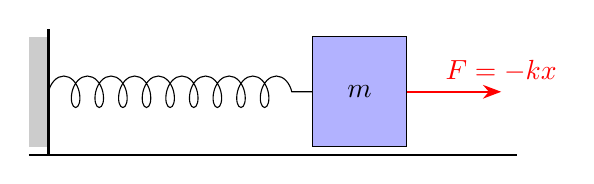
\begin{tikzpicture}
  \fill[gray!40] (0,0) rectangle (0.25,1.4);
  \draw[thick] (0.25,-0.1) -- (0.25,1.5);
  \draw[thick] (0,-0.1) -- (6.2,-0.1);
  \draw[decorate,decoration={coil,aspect=0.6,segment length=3mm,amplitude=2mm}] (0.25,0.7) -- (3.6,0.7);
  \fill[blue!30,draw=black] (3.6,0) rectangle (4.8,1.4);
  \node at (4.2,0.7) {$m$};
  \draw[-{Stealth},thick,red] (4.8,0.7) -- (6,0.7) node[above] {$F=-kx$};
\end{tikzpicture}
\caption{Masa unida a un resorte.}
\end{figure}

\subsection{Electromagnetismo}

Las cuatro ecuaciones de Maxwell, escritas con el paquete \texttt{physics}:

\begin{align*}
\divergence\vb{E} &= \frac{\rho}{\varepsilon_0} \\
\divergence\vb{B} &= 0 \\
\curl\vb{E} &= -\pdv{\vb{B}}{t} \\
\curl\vb{B} &= \mu_0\qty(\vb{J}+\varepsilon_0\pdv{\vb{E}}{t})
\end{align*}

La fuerza de Lorentz, la velocidad de la luz y el vector de Poynting:

\[ \vb{F}=q\qty(\vb{E}+\vb{v}\times\vb{B}) \qquad c=\frac{1}{\sqrt{\mu_0\varepsilon_0}} \qquad \vb{S}=\frac{1}{\mu_0}\vb{E}\times\vb{B} \]

\begin{figure}
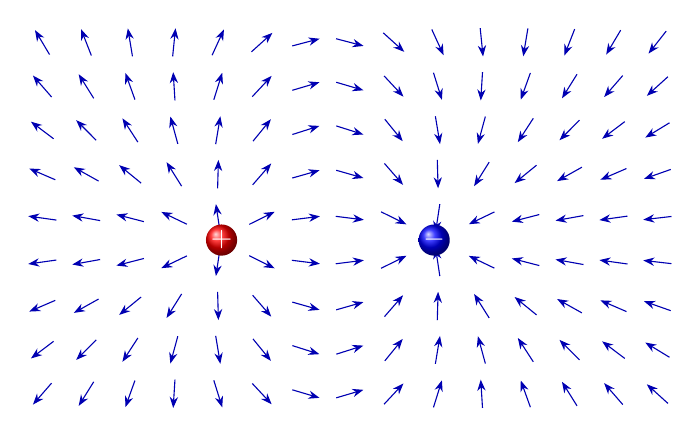
\begin{tikzpicture}[scale=0.9]
  \foreach \i in {-7,...,7} {
    \foreach \j in {-4,...,4} {
      \pgfmathsetmacro{\x}{\i*0.62+0.31}
      \pgfmathsetmacro{\y}{\j*0.62+0.31}
      \pgfmathsetmacro{\ra}{sqrt((\x-1.5)^2+(\y)^2)}
      \pgfmathsetmacro{\rb}{sqrt((\x+1.5)^2+(\y)^2)}
      \pgfmathsetmacro{\ex}{(\x+1.5)/\rb^3-(\x-1.5)/\ra^3}
      \pgfmathsetmacro{\ey}{\y/\rb^3-\y/\ra^3}
      \pgfmathsetmacro{\m}{sqrt((\ex)^2+(\ey)^2)}
      \draw[-{Stealth[length=1.4mm]},blue!70!black] (\x-0.2*\ex/\m,\y-0.2*\ey/\m) -- (\x+0.2*\ex/\m,\y+0.2*\ey/\m);
    }
  }
  \shade[ball color=red] (-1.5,0) circle (0.22);
  \shade[ball color=blue] (1.5,0) circle (0.22);
  \node[white] at (-1.5,0) {$+$};
  \node[white] at (1.5,0) {$-$};
\end{tikzpicture}
\caption{Campo eléctrico de un dipolo: cada flecha sale de calcular el campo en ese punto.}
\end{figure}

\subsection{Termodinámica}

\[ dU=\delta Q-\delta W \qquad S=k_B\ln\Omega \qquad pV=nRT \]

\[ \eta_{\text{Carnot}}=1-\frac{T_c}{T_h} \qquad B_\nu(T)=\frac{2h\nu^3}{c^2}\frac{1}{e^{h\nu/k_BT}-1} \]

\begin{figure}
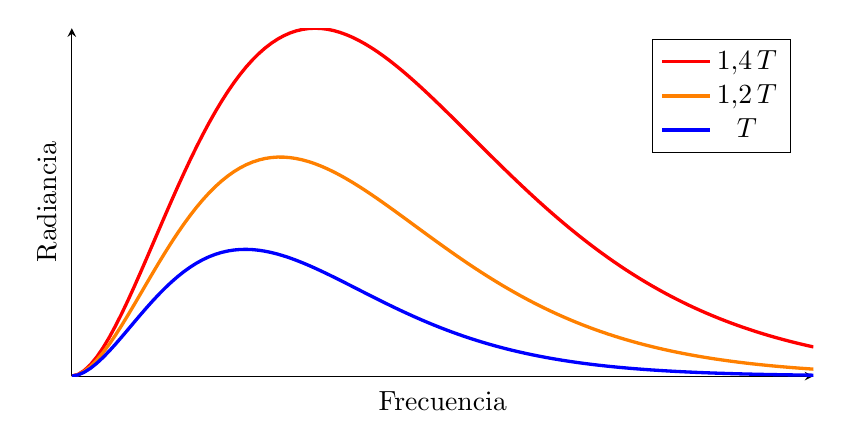
\begin{tikzpicture}
  \begin{axis}[xlabel=Frecuencia,ylabel=Radiancia,width=11cm,height=6cm,axis lines=left,xtick=\empty,ytick=\empty,ymin=0,legend pos=north east]
    \addplot[red,very thick,domain=0.02:12,samples=120] {x^3/(exp(x/1.4)-1)};
    \addplot[orange,very thick,domain=0.02:12,samples=120] {x^3/(exp(x/1.2)-1)};
    \addplot[blue,very thick,domain=0.02:12,samples=120] {x^3/(exp(x)-1)};
    \legend{$1{,}4\,T$,$1{,}2\,T$,$T$}
  \end{axis}
\end{tikzpicture}
\caption{Ley de Planck: al calentar un cuerpo negro, el máximo crece y se desplaza a frecuencias mayores.}
\end{figure}

\begin{figure}
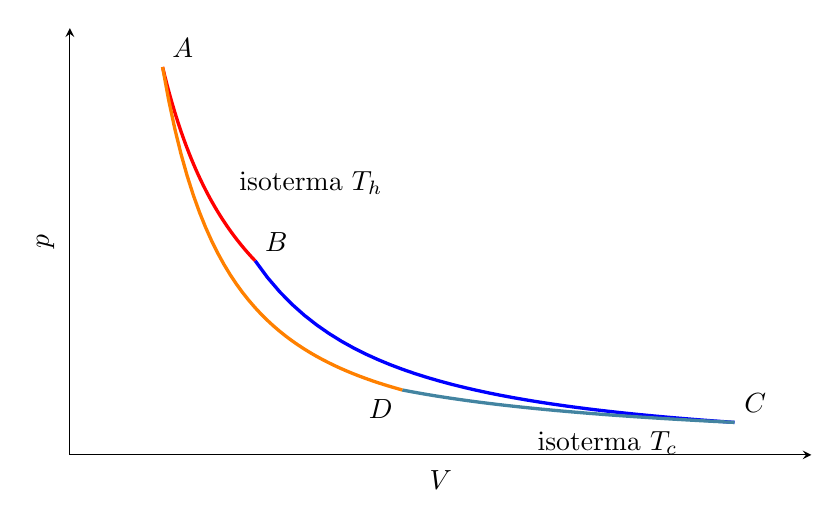
\begin{tikzpicture}
  \begin{axis}[xlabel=$V$,ylabel=$p$,width=11cm,height=7cm,axis lines=left,xmin=0,xmax=8,ymin=0,ymax=11,xtick=\empty,ytick=\empty]
    \addplot[red,very thick,domain=1:2,samples=40] {10/x};
    \addplot[blue,very thick,domain=2:7.17,samples=40] {13.195/x^1.4};
    \addplot[cyan!60!black,very thick,domain=3.586:7.17,samples=40] {6/x};
    \addplot[orange,very thick,domain=1:3.586,samples=40] {10/x^1.4};
    \node[above right] at (axis cs:1,10) {$A$};
    \node[above right] at (axis cs:2,5) {$B$};
    \node[above right] at (axis cs:7.17,0.84) {$C$};
    \node[below left] at (axis cs:3.586,1.67) {$D$};
    \node at (axis cs:2.6,7) {isoterma $T_h$};
    \node at (axis cs:5.8,0.3) {isoterma $T_c$};
  \end{axis}
\end{tikzpicture}
\caption{Ciclo de Carnot: dos isotermas y dos adiabáticas, con $\gamma=1{,}4$.}
\end{figure}

\subsection{Relatividad}

\[ \gamma=\frac{1}{\sqrt{1-v^2/c^2}} \qquad x'=\gamma(x-vt) \qquad t'=\gamma\qty(t-\frac{vx}{c^2}) \]

\[ E^2=(pc)^2+\qty(mc^2)^2 \]

\[ G_{\mu\nu}+\Lambda g_{\mu\nu}=\frac{8\pi G}{c^4}T_{\mu\nu} \]

\[ \Gamma^\lambda_{\mu\nu}=\frac{1}{2}g^{\lambda\sigma}\qty(\partial_\mu g_{\sigma\nu}+\partial_\nu g_{\sigma\mu}-\partial_\sigma g_{\mu\nu}) \]

\[ ds^2=-\qty(1-\frac{r_s}{r})c^2dt^2+\frac{dr^2}{1-r_s/r}+r^2d\Omega^2 \]

\begin{figure}
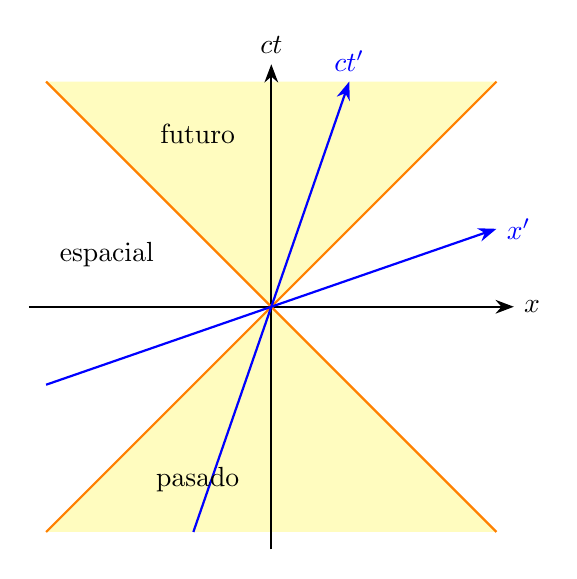
\begin{tikzpicture}[scale=1.1]
  \fill[yellow!25] (0,0) -- (2.6,2.6) -- (-2.6,2.6) -- cycle;
  \fill[yellow!25] (0,0) -- (2.6,-2.6) -- (-2.6,-2.6) -- cycle;
  \draw[-{Stealth},thick] (-2.8,0) -- (2.8,0) node[right] {$x$};
  \draw[-{Stealth},thick] (0,-2.8) -- (0,2.8) node[above] {$ct$};
  \draw[orange,thick] (-2.6,-2.6) -- (2.6,2.6);
  \draw[orange,thick] (-2.6,2.6) -- (2.6,-2.6);
  \draw[-{Stealth},thick,blue] (-0.9,-2.6) -- (0.9,2.6) node[above] {$ct'$};
  \draw[-{Stealth},thick,blue] (-2.6,-0.9) -- (2.6,0.9) node[right] {$x'$};
  \node at (-0.85,2) {futuro};
  \node at (-0.85,-2) {pasado};
  \node at (-1.9,0.6) {espacial};
\end{tikzpicture}
\caption{Diagrama de Minkowski: el cono de luz y los ejes de un observador en movimiento.}
\end{figure}

\subsection{Mecánica cuántica}

\[ i\hbar\pdv{\psi}{t}=-\frac{\hbar^2}{2m}\laplacian\psi+V\psi \]

\[ \Delta x\,\Delta p\ge\frac{\hbar}{2} \qquad \comm{\hat{x}}{\hat{p}}=i\hbar \qquad E_n=\frac{n^2\pi^2\hbar^2}{2mL^2} \]

\[ \ket{\psi}=\alpha\ket{0}+\beta\ket{1} \qquad \braket{\psi}{\phi} \qquad \expval{A}{\psi} \]

\[ (i\gamma^\mu\partial_\mu-m)\psi=0 \]

\[ \sigma_x=\begin{pmatrix} 0 & 1 \\ 1 & 0 \end{pmatrix} \qquad \sigma_y=\begin{pmatrix} 0 & -i \\ i & 0 \end{pmatrix} \qquad \sigma_z=\begin{pmatrix} 1 & 0 \\ 0 & -1 \end{pmatrix} \]

\[ \mathcal{L}=\bar{\psi}\qty(i\gamma^\mu D_\mu-m)\psi-\frac{1}{4}F_{\mu\nu}F^{\mu\nu} \]

\begin{figure}
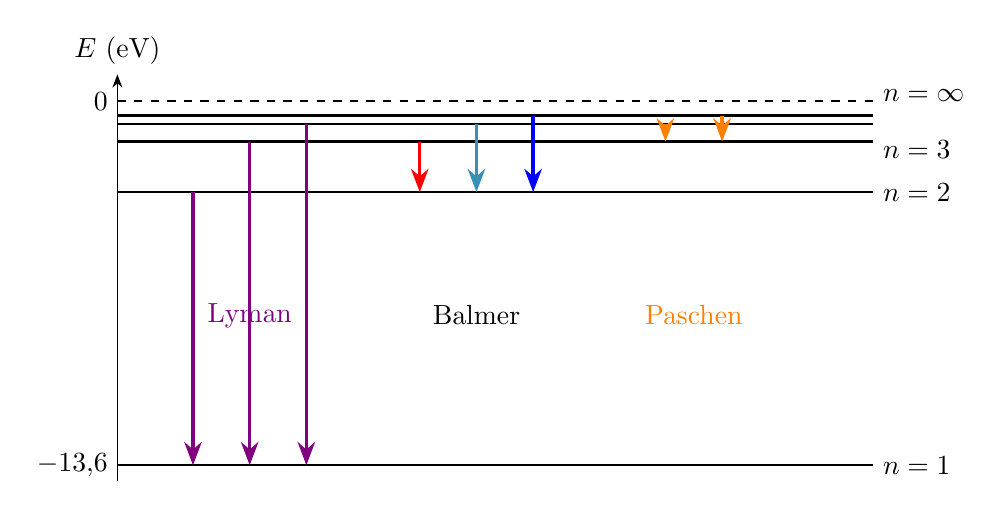
\begin{tikzpicture}[yscale=0.34,xscale=1.2]
  \draw[-{Stealth}] (0,-14.2) -- (0,1) node[above] {$E$ (\si{eV})};
  \foreach \n/\e in {1/-13.6,2/-3.4,3/-1.51,4/-0.85,5/-0.54} {
    \draw[thick] (0,\e) -- (8,\e);
  }
  \foreach \n/\e in {1/-13.6,2/-3.4,3/-1.8} {
    \node[right] at (8,\e) {$n=\n$};
  }
  \node[right] at (8,0.2) {$n=\infty$};
  \draw[thick,dashed] (0,0) -- (8,0);
  \node[left] at (0,0) {$0$};
  \node[left] at (0,-13.6) {$-13{,}6$};
  \foreach \x/\a/\c in {0.8/2/violet,1.4/3/violet,2/4/violet} {
    \draw[-{Stealth},very thick,\c] (\x,{-13.6/\a/\a}) -- (\x,-13.6);
  }
  \foreach \x/\a/\c in {3.2/3/red,3.8/4/cyan!70!black,4.4/5/blue} {
    \draw[-{Stealth},very thick,\c] (\x,{-13.6/\a/\a}) -- (\x,-3.4);
  }
  \foreach \x/\a in {5.8/4,6.4/5} {
    \draw[-{Stealth},very thick,orange] (\x,{-13.6/\a/\a}) -- (\x,-1.51);
  }
  \node[violet] at (1.4,-8) {Lyman};
  \node at (3.8,-8) {Balmer};
  \node[orange] at (6.1,-8) {Paschen};
\end{tikzpicture}
\caption{Niveles del átomo de hidrógeno, $E_n=-13{,}6/n^2$, y sus series espectrales.}
\end{figure}

\begin{figure}
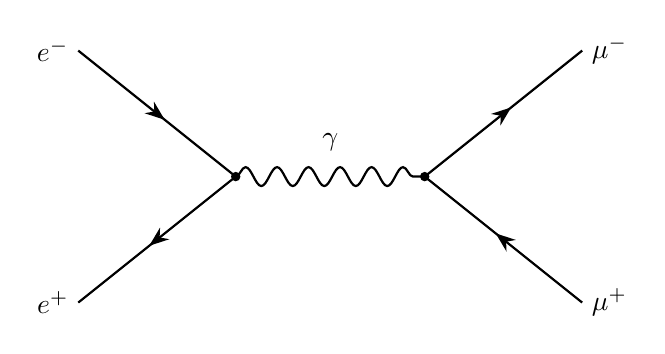
\begin{tikzpicture}[fermion/.style={thick,postaction={decorate},decoration={markings,mark=at position 0.55 with {\arrow{Stealth[length=2.5mm]}}}},foton/.style={thick,decorate,decoration={snake,amplitude=1.2mm,segment length=4mm}}]
  \coordinate (a) at (0,1.6);
  \coordinate (b) at (0,-1.6);
  \coordinate (v1) at (2,0);
  \coordinate (v2) at (4.4,0);
  \coordinate (c) at (6.4,1.6);
  \coordinate (d) at (6.4,-1.6);
  \draw[fermion] (a) -- (v1);
  \draw[fermion] (v1) -- (b);
  \draw[foton] (v1) -- (v2);
  \draw[fermion] (v2) -- (c);
  \draw[fermion] (d) -- (v2);
  \fill (v1) circle (0.06);
  \fill (v2) circle (0.06);
  \node[left] at (a) {$e^-$};
  \node[left] at (b) {$e^+$};
  \node[right] at (c) {$\mu^-$};
  \node[right] at (d) {$\mu^+$};
  \node[above] at (3.2,0.2) {$\gamma$};
\end{tikzpicture}
\caption{Diagrama de Feynman: un electrón y un positrón se aniquilan y crean un par de muones.}
\end{figure}

\subsection{Ondas y óptica}

\[ \pdv[2]{u}{t}=c^2\pdv[2]{u}{x} \qquad n_1\sin\theta_1=n_2\sin\theta_2 \qquad \frac{1}{f}=\frac{1}{d_o}+\frac{1}{d_i} \]

\begin{figure}
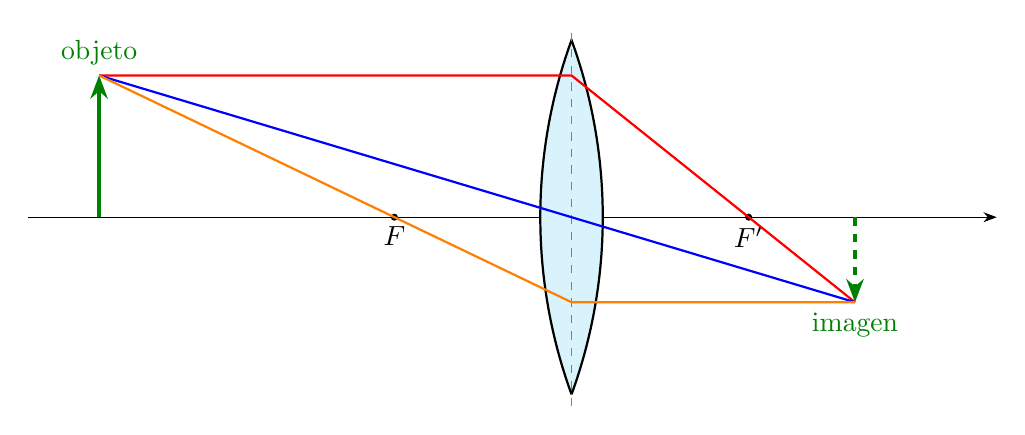
\begin{tikzpicture}[scale=1.5]
  \draw[-{Stealth}] (-4.6,0) -- (3.6,0);
  \draw[thick,fill=cyan!15] (0,-1.5) arc (-20:20:4.385) arc (160:200:4.385);
  \draw[dashed,gray] (0,-1.6) -- (0,1.6);
  \fill (-1.5,0) circle (0.03) node[below] {$F$};
  \fill (1.5,0) circle (0.03) node[below] {$F'$};
  \draw[-{Stealth},very thick,green!50!black] (-4,0) -- (-4,1.2) node[above] {objeto};
  \draw[-{Stealth},very thick,green!50!black,dashed] (2.4,0) -- (2.4,-0.72) node[below] {imagen};
  \draw[red,thick] (-4,1.2) -- (0,1.2) -- (2.4,-0.72);
  \draw[blue,thick] (-4,1.2) -- (2.4,-0.72);
  \draw[orange,thick] (-4,1.2) -- (0,-0.72) -- (2.4,-0.72);
\end{tikzpicture}
\caption{Lente convergente de $f=\SI{1.5}{cm}$: los tres rayos notables se cortan en la imagen.}
\end{figure}

\subsection{Unidades y constantes}

\begin{tabular}{lcr}
\hline
\textbf{Constante} & \textbf{Símbolo} & \textbf{Valor} \\
\hline
Velocidad de la luz & $c$ & \SI{299792458}{m/s} \\
Constante de Planck & $h$ & \SI{6.62607015e-34}{\joule\second} \\
Carga elemental & $e$ & \SI{1.602176634e-19}{C} \\
Constante de Boltzmann & $k_B$ & \SI{1.380649e-23}{J/K} \\
Número de Avogadro & $N_A$ & \SI{6.02214076e23}{mol^{-1}} \\
\hline
\end{tabular}

\section{Química}

\subsection{Reacciones}

Combustión, síntesis y descomposición:

\[ \ce{CH4 + 2O2 -> CO2 + 2H2O} \]

\[ \ce{N2 + 3H2 <=>[Fe][450 ^\circ C] 2NH3} \]

\[ \ce{CaCO3 ->[\Delta] CaO + CO2 ^} \]

\[ \ce{6CO2 + 6H2O ->[h\nu] C6H12O6 + 6O2} \]

Disoluciones, ácidos y bases, oxidación y reducción:

\[ \ce{Ag+ + Cl- -> AgCl v} \]

\[ \ce{CH3COOH + H2O <=> CH3COO- + H3O+} \]

\[ \ce{Zn + Cu^2+ -> Zn^2+ + Cu} \]

\[ \ce{2MnO4- + 5H2C2O4 + 6H+ -> 2Mn^2+ + 10CO2 ^ + 8H2O} \]

Compuestos de coordinación, hidratos y reacciones nucleares:

\[ \ce{[Cu(NH3)4]^2+} \qquad \ce{CuSO4*5H2O} \qquad \ce{K4[Fe(CN)6]} \]

\[ \ce{^{235}_{92}U + ^1_0n -> ^{141}_{56}Ba + ^{92}_{36}Kr + 3 ^1_0n} \]

\subsection{Moléculas}

\begin{tabular}[cabecera=no,filas=no]{ccc}
Metano & Etanol & Ácido acético \\
\chemfig{C(-[:0]H)(-[:90]H)(-[:180]H)(-[:270]H)} & \chemfig{H_3C-CH_2-OH} & \chemfig{CH_3-C(=[1]O)-[7]OH} \\
Etileno & Acetileno & Urea \\
\chemfig{H_2C=CH_2} & \chemfig{HC~CH} & \chemfig{H_2N-C(=[2]O)-NH_2} \\
\end{tabular}

Los anillos aromáticos y las moléculas biológicas:

\[ \chemfig{*6(=-=-=-)} \qquad \chemfig{*6(-=-=-=)} \qquad \chemfig{*6(=-=(-OH)-=-)} \]

\begin{figure}
\[ \chemfig{*6(=-=(-O-[:-30](=[:-90]O)-[:30]CH_3)-(-[:30](=[:90]O)-[:-30]OH)=-)} \]
\caption{Aspirina (ácido acetilsalicílico).}
\end{figure}

\begin{figure}
\[ \chemfig{*6((=O)-N(-CH_3)-*5(-N=-N(-CH_3)-=)--(=O)-N(-H_3C)-)} \]
\caption{Cafeína.}
\end{figure}

\begin{figure}
\[ \chemfig{*6(=N-*5(-N(-H)-=N-)=-(-NH_2)=N-)} \qquad \chemfig{O*6(-(-OH)-(-OH)-(-OH)-(-OH)-(-CH_2OH)-)} \qquad \chemfig{H_2N-CH_2-C(=[1]O)-[7]OH} \]
\caption{Adenina, glucosa y glicina.}
\end{figure}

\subsection{Esquemas}

\[ \schemestart A \arrow{->} B \arrow{<=>} C \arrow{->[catalizador][calor]} D \schemestop \]

\subsection{Equilibrio y cinética}

\[ K_c=\frac{[\ce{C}]^c[\ce{D}]^d}{[\ce{A}]^a[\ce{B}]^b} \qquad \mathrm{pH}=\mathrm{p}K_a+\log_{10}\frac{[\ce{A-}]}{[\ce{HA}]} \]

\[ k=A\,e^{-E_a/RT} \qquad E=E^\circ-\frac{RT}{nF}\ln Q \qquad \Delta G=\Delta H-T\Delta S \]

\begin{figure}
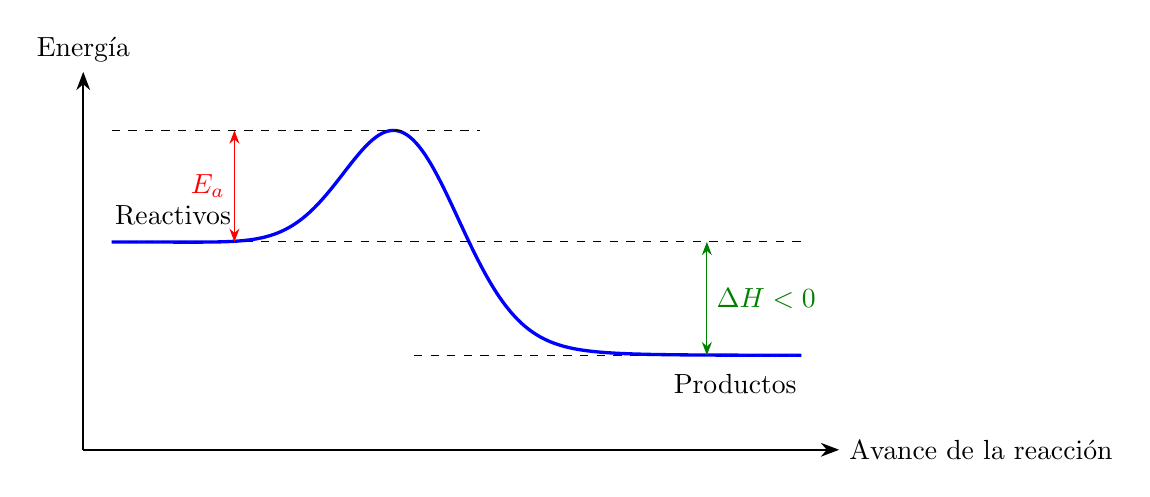
\begin{tikzpicture}[scale=1.2]
  \draw[-{Stealth},thick] (0,0) -- (0,4) node[above] {Energía};
  \draw[-{Stealth},thick] (0,0) -- (8,0) node[right] {Avance de la reacción};
  \draw[very thick,blue] plot[domain=0.3:7.6,samples=120,smooth] (\x,{2.2-1.2/(1+exp(-2.2*(\x-3.8)))+1.5*exp(-1.4*(\x-3.4)^2)});
  \draw[dashed] (0.3,2.2) -- (7.6,2.2);
  \draw[dashed] (3.5,1) -- (7.6,1);
  \draw[dashed] (0.3,3.38) -- (4.2,3.38);
  \draw[{Stealth}-{Stealth},red] (1.6,2.2) -- (1.6,3.38) node[midway,left] {$E_a$};
  \draw[{Stealth}-{Stealth},green!50!black] (6.6,2.2) -- (6.6,1) node[midway,right] {$\Delta H<0$};
  \node at (0.95,2.48) {Reactivos};
  \node at (6.9,0.7) {Productos};
\end{tikzpicture}
\caption{Perfil de una reacción exotérmica.}
\end{figure}

\subsection{Tabla periódica}

La tabla periódica es una extensión de las tablas: la misma rejilla, con huecos, un color por familia y los 118 elementos.

\tablaperiodica

Sus colores, sus líneas y su tamaño son opciones. Esta enseña los tres primeros periodos con nombres y masas, y cambia el color de dos familias:

\tablaperiodica[periodos=3,nombres=si,masas=si,nobles=violet!35,alcalinos=red!35,leyenda=no]

Como es una tabla más, también se puede escribir a mano:

\begin{tabular}[cabecera=no,filas=no,vacias=no,columnas=iguales,proporcion=1.1,ancho=natural]{cccc}
\cellcolor{red!20}\makecell{\tiny 3\\\textbf{Li}} & & & \cellcolor{cyan!25}\makecell{\tiny 10\\\textbf{Ne}} \\
\cellcolor{red!20}\makecell{\tiny 11\\\textbf{Na}} & \cellcolor{orange!25}\makecell{\tiny 12\\\textbf{Mg}} & & \cellcolor{cyan!25}\makecell{\tiny 18\\\textbf{Ar}} \\
\end{tabular}

\section{Diagramas}

\subsection{Diagrama de flujo}

\begin{figure}
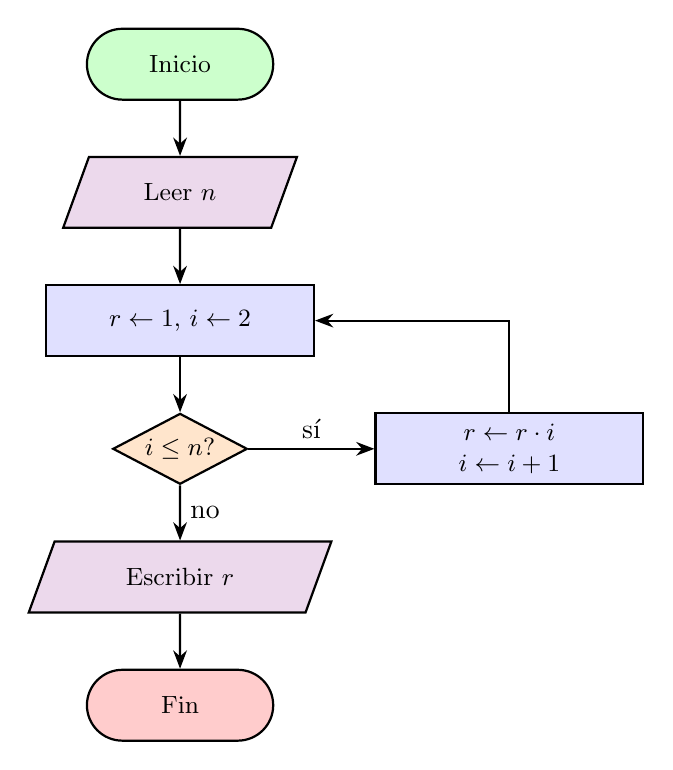
\begin{tikzpicture}[node distance=7mm and 16mm,
  base/.style={draw,thick,minimum height=9mm,align=center,font=\small},
  inicio/.style={base,rounded rectangle,fill=green!20,minimum width=26mm},
  proceso/.style={base,rectangle,fill=blue!12,minimum width=34mm},
  decision/.style={base,diamond,aspect=2.2,fill=orange!20,inner sep=1pt},
  dato/.style={base,trapezium,trapezium left angle=70,trapezium right angle=110,fill=violet!15,minimum width=26mm},
  flecha/.style={-{Stealth},thick}]
  \node[inicio] (a) {Inicio};
  \node[dato,below=of a] (b) {Leer $n$};
  \node[proceso,below=of b] (c) {$r\gets 1$, $i\gets 2$};
  \node[decision,below=of c] (d) {$i\le n$?};
  \node[proceso,right=of d] (e) {$r\gets r\cdot i$\\$i\gets i+1$};
  \node[dato,below=of d] (f) {Escribir $r$};
  \node[inicio,below=of f,fill=red!20] (g) {Fin};
  \draw[flecha] (a) -- (b);
  \draw[flecha] (b) -- (c);
  \draw[flecha] (c) -- (d);
  \draw[flecha] (d) -- node[above] {sí} (e);
  \draw[flecha] (d) -- node[right] {no} (f);
  \draw[flecha] (f) -- (g);
  \draw[flecha] (e) |- (c);
\end{tikzpicture}
\caption{Cálculo del factorial con un bucle.}
\end{figure}

\begin{figure}
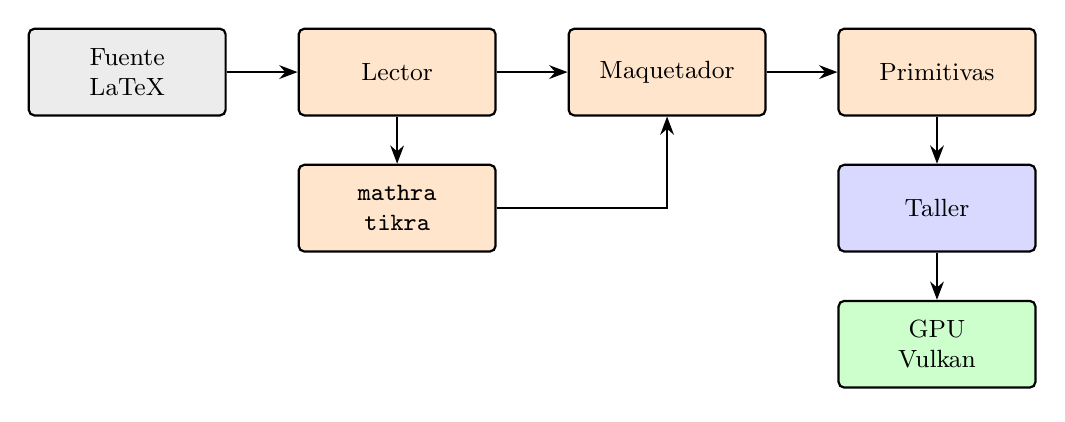
\begin{tikzpicture}[node distance=6mm and 9mm,
  caja/.style={draw,thick,rounded corners=2pt,minimum width=25mm,minimum height=11mm,align=center,font=\small},
  r/.style={caja,fill=orange!20},
  c/.style={caja,fill=blue!15},
  g/.style={caja,fill=green!20},
  flecha/.style={-{Stealth},thick}]
  \node[caja,fill=gray!15] (f) {Fuente\\LaTeX};
  \node[r,right=of f] (l) {Lector};
  \node[r,right=of l] (m) {Maquetador};
  \node[r,right=of m] (p) {Primitivas};
  \node[r,below=of l] (a) {\texttt{mathra}\\\texttt{tikra}};
  \node[c,below=of p] (t) {Taller};
  \node[c,left=of t,xshift=-34mm,yshift=-18mm,opacity=0] (o) {};
  \node[g,below=of t] (g) {GPU\\Vulkan};
  \draw[flecha] (f) -- (l);
  \draw[flecha] (l) -- (m);
  \draw[flecha] (m) -- (p);
  \draw[flecha] (l) -- (a);
  \draw[flecha] (a) -| (m);
  \draw[flecha] (p) -- (t);
  \draw[flecha] (t) -- (g);
\end{tikzpicture}
\caption{El camino de una fuente hasta la pantalla en este mismo motor.}
\end{figure}

\begin{figure}
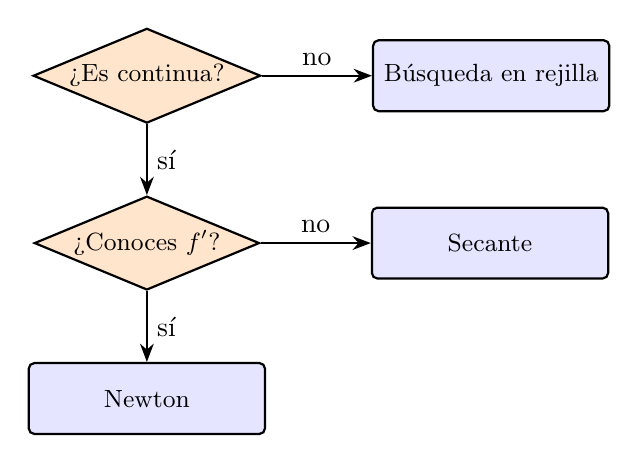
\begin{tikzpicture}[node distance=9mm and 14mm,
  c/.style={draw,thick,rectangle,rounded corners=2pt,minimum width=30mm,minimum height=9mm,align=center,font=\small,fill=blue!10},
  d/.style={draw,thick,diamond,aspect=2.4,inner sep=1pt,align=center,font=\small,fill=orange!20},
  f/.style={-{Stealth},thick}]
  \node[d] (a) {¿Es continua?};
  \node[d,below=of a] (b) {¿Conoces $f'$?};
  \node[c,right=of a] (x) {Búsqueda en rejilla};
  \node[c,below=of b] (n) {Newton};
  \node[c,right=of b] (s) {Secante};
  \draw[f] (a) -- node[above] {no} (x);
  \draw[f] (a) -- node[right] {sí} (b);
  \draw[f] (b) -- node[above] {no} (s);
  \draw[f] (b) -- node[right] {sí} (n);
\end{tikzpicture}
\caption{Un árbol de decisión con varias salidas.}
\end{figure}

\subsection{Máquina de estados}

\begin{figure}
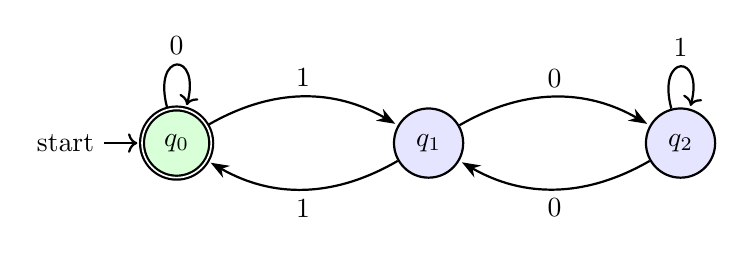
\begin{tikzpicture}[shorten >=1pt,node distance=3.2cm,on grid,auto,thick]
  \node[state,initial,accepting,fill=green!15] (q0) {$q_0$};
  \node[state,fill=blue!10,right=of q0] (q1) {$q_1$};
  \node[state,fill=blue!10,right=of q1] (q2) {$q_2$};
  \path[-{Stealth}]
    (q0) edge[loop above] node {0} ()
         edge[bend left] node {1} (q1)
    (q1) edge[bend left] node {1} (q0)
         edge[bend left] node {0} (q2)
    (q2) edge[bend left] node {0} (q1)
         edge[loop above] node {1} ();
\end{tikzpicture}
\caption{Autómata que acepta los binarios múltiplos de 3.}
\end{figure}

\subsection{Árboles}

\begin{figure}
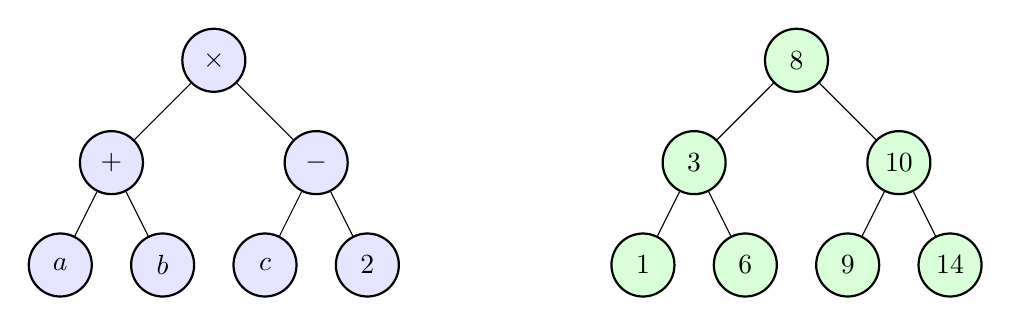
\begin{tikzpicture}[level distance=13mm,sibling distance=26mm,every node/.style={circle,draw,thick,minimum size=8mm,fill=blue!10},level 2/.style={sibling distance=13mm}]
  \node {$\times$}
    child {node {$+$}
      child {node {$a$}}
      child {node {$b$}}}
    child {node {$-$}
      child {node {$c$}}
      child {node {$2$}}};
  \begin{scope}[xshift=7.4cm,every node/.style={circle,draw,thick,minimum size=8mm,fill=green!15}]
    \node {8}
      child {node {3}
        child {node {1}}
        child {node {6}}}
      child {node {10}
        child {node {9}}
        child {node {14}}};
  \end{scope}
\end{tikzpicture}
\caption{Árbol sintáctico de $(a+b)\times(c-2)$ y árbol binario de búsqueda.}
\end{figure}

\subsection{Grafos}

\begin{figure}
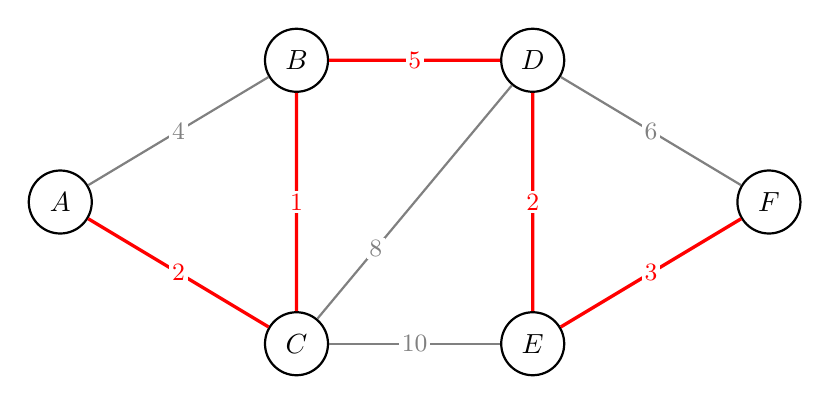
\begin{tikzpicture}[scale=1.2,v/.style={circle,draw,thick,minimum size=8mm,fill=white},p/.style={font=\small,fill=white,inner sep=1pt},cam/.style={very thick,red}]
  \node[v] (A) at (0,1.5) {$A$};
  \node[v] (B) at (2.5,3) {$B$};
  \node[v] (C) at (2.5,0) {$C$};
  \node[v] (D) at (5,3) {$D$};
  \node[v] (E) at (5,0) {$E$};
  \node[v] (F) at (7.5,1.5) {$F$};
  \draw[thick,gray] (A) -- node[p] {4} (B);
  \draw[cam] (A) -- node[p] {2} (C);
  \draw[cam] (C) -- node[p] {1} (B);
  \draw[cam] (B) -- node[p] {5} (D);
  \draw[thick,gray] (C) -- node[p,pos=0.3] {8} (D);
  \draw[thick,gray] (C) -- node[p] {10} (E);
  \draw[cam] (D) -- node[p] {2} (E);
  \draw[thick,gray] (D) -- node[p] {6} (F);
  \draw[cam] (E) -- node[p] {3} (F);
\end{tikzpicture}
\caption{Grafo con pesos: en rojo, el camino más corto de $A$ a $F$, de coste 13.}
\end{figure}

\subsection{Redes neuronales}

\begin{figure}
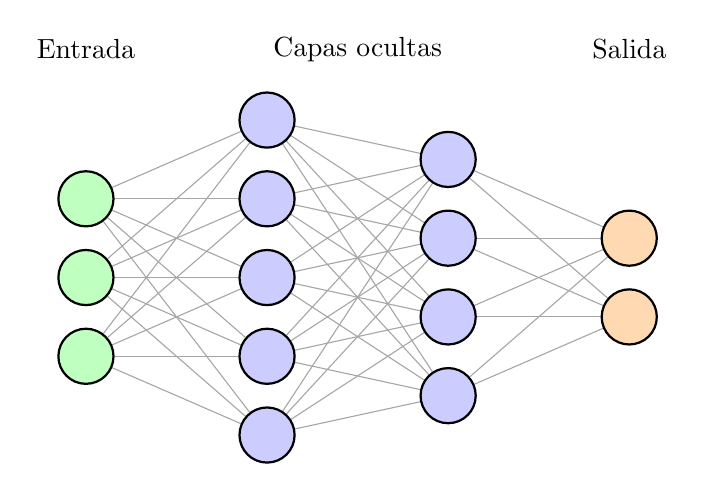
\begin{tikzpicture}[x=2.3cm,y=1cm,n/.style={circle,draw,thick,minimum size=7mm,inner sep=0pt}]
  \foreach \i in {1,...,3} { \node[n,fill=green!25] (a\i) at (0,\i-2) {}; }
  \foreach \i in {1,...,5} { \node[n,fill=blue!20] (b\i) at (1,\i-3) {}; }
  \foreach \i in {1,...,4} { \node[n,fill=blue!20] (c\i) at (2,\i-2.5) {}; }
  \foreach \i in {1,...,2} { \node[n,fill=orange!30] (d\i) at (3,\i-1.5) {}; }
  \begin{scope}[on background layer]
    \foreach \i in {1,...,3} { \foreach \j in {1,...,5} { \draw[gray!70] (a\i) -- (b\j); } }
    \foreach \i in {1,...,5} { \foreach \j in {1,...,4} { \draw[gray!70] (b\i) -- (c\j); } }
    \foreach \i in {1,...,4} { \foreach \j in {1,...,2} { \draw[gray!70] (c\i) -- (d\j); } }
  \end{scope}
  \node at (0,2.9) {Entrada};
  \node at (1.5,2.9) {Capas ocultas};
  \node at (3,2.9) {Salida};
\end{tikzpicture}
\caption{Perceptrón con dos capas ocultas.}
\end{figure}

\subsection{Secuencias}

\begin{figure}
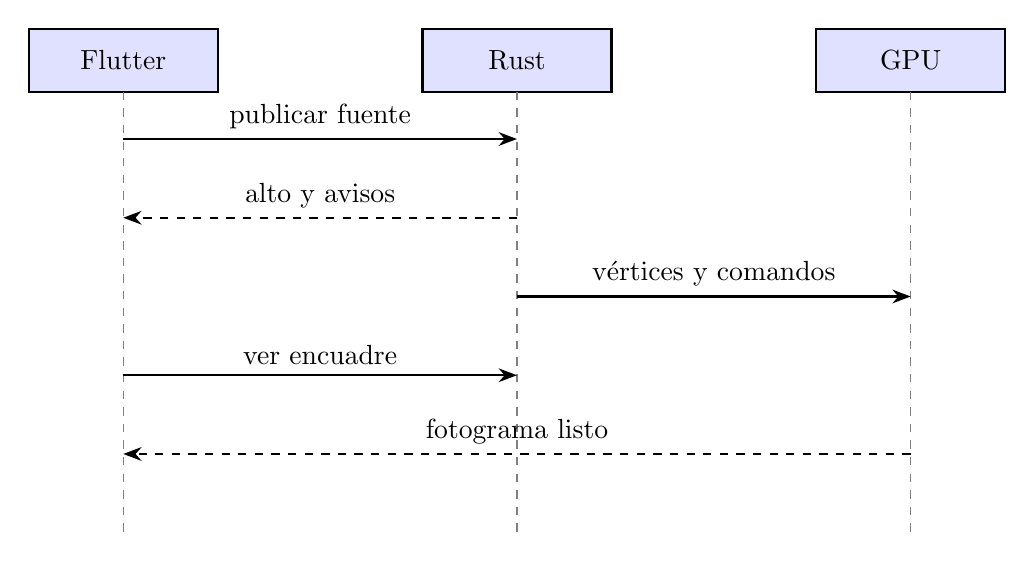
\begin{tikzpicture}[x=1cm,y=1cm,c/.style={draw,thick,fill=blue!12,minimum width=24mm,minimum height=8mm},m/.style={-{Stealth},thick}]
  \node[c] (a) at (0,0) {Flutter};
  \node[c] (b) at (5,0) {Rust};
  \node[c] (d) at (10,0) {GPU};
  \foreach \x in {0,5,10} { \draw[dashed,gray] (\x,-0.4) -- (\x,-6); }
  \draw[m] (0,-1) -- node[above] {publicar fuente} (5,-1);
  \draw[m,dashed] (5,-2) -- node[above] {alto y avisos} (0,-2);
  \draw[m] (5,-3) -- node[above] {vértices y comandos} (10,-3);
  \draw[m] (0,-4) -- node[above] {ver encuadre} (5,-4);
  \draw[m,dashed] (10,-5) -- node[above] {fotograma listo} (0,-5);
\end{tikzpicture}
\caption{Diagrama de secuencia de un fotograma.}
\end{figure}

\subsection{Mapas conceptuales y conjuntos}

\begin{figure}
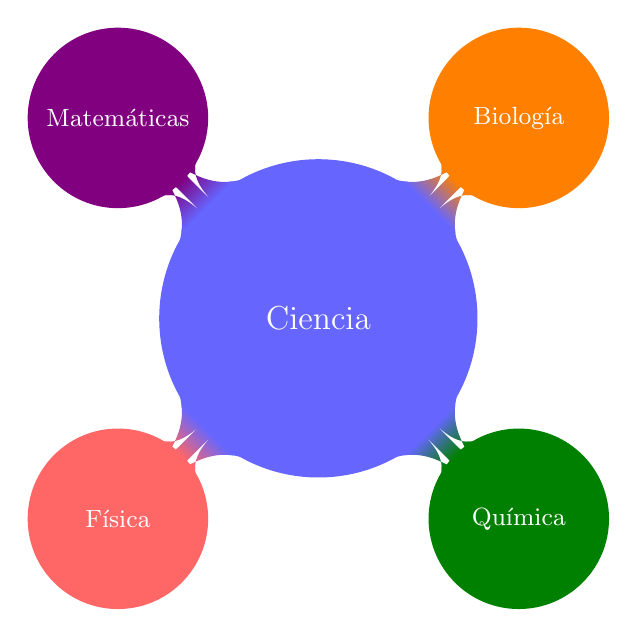
\begin{tikzpicture}[mindmap,grow cyclic,concept color=blue!60,every node/.style={concept,text=white},level 1/.append style={level distance=36mm,sibling angle=90},level 2/.append style={level distance=24mm,sibling angle=45}]
  \node {Ciencia}
    child[concept color=red!60] {node {Física}}
    child[concept color=green!50!black] {node {Química}}
    child[concept color=orange] {node {Biología}}
    child[concept color=violet] {node {Matemáticas}};
\end{tikzpicture}
\caption{Mapa conceptual.}
\end{figure}

\begin{figure}
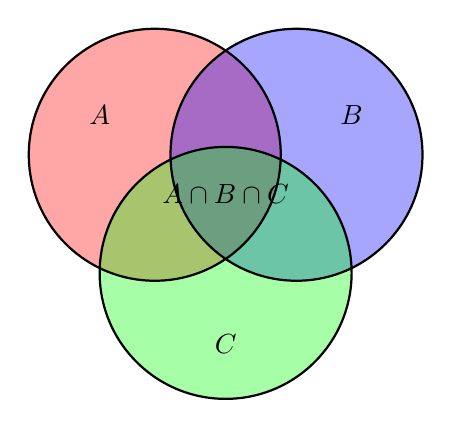
\begin{tikzpicture}
  \fill[red,fill opacity=0.35] (0,0) circle (1.6);
  \fill[blue,fill opacity=0.35] (1.8,0) circle (1.6);
  \fill[green,fill opacity=0.35] (0.9,-1.5) circle (1.6);
  \draw[thick] (0,0) circle (1.6);
  \draw[thick] (1.8,0) circle (1.6);
  \draw[thick] (0.9,-1.5) circle (1.6);
  \node at (-0.7,0.5) {$A$};
  \node at (2.5,0.5) {$B$};
  \node at (0.9,-2.4) {$C$};
  \node at (0.9,-0.5) {$A\cap B\cap C$};
\end{tikzpicture}
\caption{Diagrama de Venn con transparencias.}
\end{figure}

\subsection{Calendario de un proyecto}

\begin{figure}
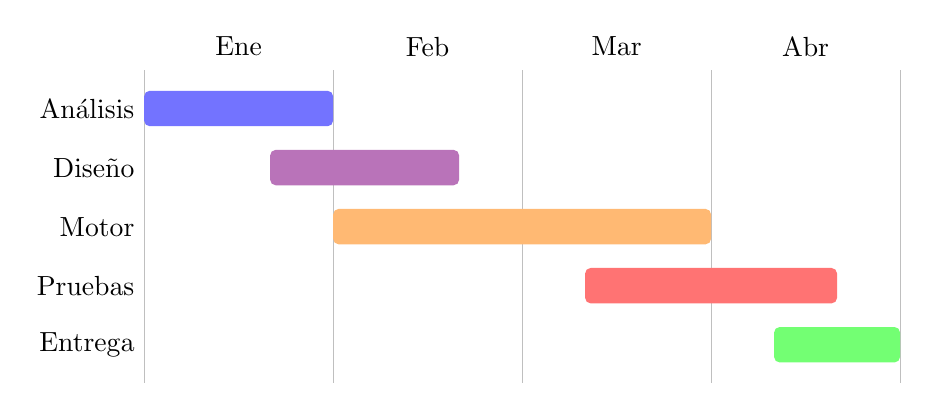
\begin{tikzpicture}[x=0.8cm,y=0.75cm]
  \foreach \m/\n in {0/Ene,3/Feb,6/Mar,9/Abr} { \node at (\m+1.5,0.7) {\n}; }
  \foreach \x in {0,3,...,12} { \draw[gray!50] (\x,0.3) -- (\x,-5); }
  \foreach \i/\n/\d/\f/\c in {1/Análisis/0/3/blue,2/Diseño/2/5/violet,3/Motor/3/9/orange,4/Pruebas/7/11/red,5/Entrega/10/12/green} {
    \fill[\c!55,rounded corners=2pt] (\d,-\i+0.35) rectangle (\f,-\i+0.95);
    \node[left] at (0,-\i+0.65) {\n};
  }
\end{tikzpicture}
\caption{Diagrama de Gantt.}
\end{figure}

\section{Electrónica}

\begin{figure}
\begin{circuitikz}
  \draw (0,0) to[V,v=$V_0$] (0,3) to[R,l=$R$] (3,3) to[L,l=$L$] (6,3) to[C,l=$C$] (6,0) -- (0,0);
\end{circuitikz}
\caption{Circuito RLC en serie.}
\end{figure}

\begin{figure}
\begin{circuitikz}
  \draw (0,0) node[op amp] (o) {};
  \draw (o.-) to[short,-*] ++(-0.5,0) coordinate (a) to[R,l_=$R_1$] ++(-2.5,0) node[left] {$V_e$};
  \draw (a) -- ++(0,1.7) coordinate (b) to[R,l=$R_2$] (b -| o.out) -- (o.out);
  \draw (o.+) to[short] ++(-0.5,0) node[ground] {};
  \draw (o.out) to[short,-o] ++(1,0) node[right] {$V_s=-\frac{R_2}{R_1}V_e$};
\end{circuitikz}
\caption{Amplificador inversor con amplificador operacional.}
\end{figure}

\begin{figure}
\begin{circuitikz}
  \draw (0,0) to[R,l=$R_1$] (2.2,2.2) to[R,l=$R_2$] (4.4,0) to[R,l=$R_3$] (2.2,-2.2) to[R,l=$R_4$] (0,0);
  \draw (2.2,2.2) to[voltmeter] (2.2,-2.2);
  \draw (0,0) -- (-1.4,0) to[V,l=$V$] (-1.4,-3.2) -- (4.4,-3.2) -- (4.4,0);
\end{circuitikz}
\caption{Puente de Wheatstone.}
\end{figure}

\begin{figure}
\begin{circuitikz}
  \draw (0,0) node[and port] (a) {};
  \draw (0,-2) node[or port] (b) {};
  \draw (3,-1) node[xor port] (c) {};
  \draw (a.out) -| (c.in 1);
  \draw (b.out) -| (c.in 2);
\end{circuitikz}
\caption{Puertas lógicas.}
\end{figure}

\section{Animaciones}

Cada animación es una figura con un parámetro \texttt{t}: el motor la recompone en cada fotograma y solo gasta tiempo en las que se ven. Baja despacio: todas están en movimiento.

\subsection{Mecanismos}

\begin{figure}
\begin{animacion}[t=0:360, duracion=3]
\begin{tikzpicture}
  \pgfmathsetmacro{\px}{cos(\t)}
  \pgfmathsetmacro{\py}{sin(\t)}
  \pgfmathsetmacro{\lx}{\px+sqrt(9-\py*\py)}
  \pgfmathtruncatemacro{\g}{\t}
  \draw[thick] (0,0) circle (1);
  \draw (1.6,-0.7) -- (5.2,-0.7) (1.6,0.7) -- (5.2,0.7);
  \fill[gray!30,draw=black] (\lx-0.4,-0.6) rectangle (\lx+0.8,0.6);
  \draw[very thick,blue] (0,0) -- (\px,\py) -- (\lx,0);
  \fill (0,0) circle (0.06) (\px,\py) circle (0.06) (\lx,0) circle (0.06);
  \node at (0,-1.4) {$\theta=\g^\circ$};
\end{tikzpicture}
\end{animacion}
\caption{Biela y manivela: convierte giro en vaivén.}
\end{figure}

\begin{figure}
\begin{animacion}[t=0:360, duracion=4]
\begin{tikzpicture}
  \begin{scope}[rotate=\t]
    \foreach \i in {0,...,11} {
      \fill[orange!70!black,rotate=\i*30] (0.86,-0.13) -- (1.1,-0.07) -- (1.1,0.07) -- (0.86,0.13) -- cycle;
    }
    \fill[orange!80] (0,0) circle (0.9);
    \fill[white] (0,0) circle (0.18);
    \draw[orange!40!black,thick] (0,0) -- (0.8,0);
  \end{scope}
  \begin{scope}[xshift=3cm,rotate=-\t/2]
    \foreach \i in {0,...,23} {
      \fill[blue!70!black,rotate=180+7.5+\i*15] (1.86,-0.13) -- (2.1,-0.07) -- (2.1,0.07) -- (1.86,0.13) -- cycle;
    }
    \fill[blue!50] (0,0) circle (1.9);
    \fill[white] (0,0) circle (0.25);
    \draw[blue!30!black,thick] (0,0) -- (1.7,0);
  \end{scope}
\end{tikzpicture}
\end{animacion}
\caption{Engranajes de 12 y 24 dientes: el grande gira a la mitad de velocidad.}
\end{figure}

\subsection{Oscilaciones y ondas}

\begin{figure}
\begin{animacion}[t=0:360, duracion=3]
\begin{tikzpicture}
  \pgfmathsetmacro{\a}{30*cos(\t)}
  \pgfmathsetmacro{\u}{(1-cos(\a))/(1-cos(30))}
  \draw[dashed,gray] (0,0) -- (0,-3.2);
  \draw[gray] (-1.5,-2.598) arc (240:300:3);
  \fill[gray!40] (-1,0) rectangle (1,0.12);
  \draw[thick] (0,0) -- ({3*sin(\a)},{-3*cos(\a)});
  \shade[ball color=blue!70] ({3*sin(\a)},{-3*cos(\a)}) circle (0.22);
  \draw (3,-3) rectangle (3.6,0);
  \draw (4.2,-3) rectangle (4.8,0);
  \fill[red!60] (3,-3) rectangle (3.6,{-3+3*\u+0.001});
  \fill[blue!60] (4.2,-3) rectangle (4.8,{-3*\u+0.001});
  \node at (3.3,-3.3) {$U$};
  \node at (4.5,-3.3) {$K$};
\end{tikzpicture}
\end{animacion}
\caption{Péndulo: la energía pasa de potencial a cinética y su suma no cambia.}
\end{figure}

\begin{figure}
\begin{animacion}[t=0.05:20, duracion=8]
\begin{tikzpicture}
  \pgfmathsetmacro{\x}{exp(-0.15*\t)*cos(deg(2*\t))}
  \fill[gray!40] (0,-0.6) rectangle (0.2,0.6);
  \draw[decorate,decoration={coil,aspect=0.6,segment length=2.2mm,amplitude=1.5mm}] (0.2,0) -- ({2.4+\x},0);
  \fill[blue!30,draw=black] ({2.4+\x},-0.45) rectangle ({3.2+\x},0.45);
  \begin{scope}[xshift=5cm]
    \draw[->] (0,0) -- (6.4,0) node[right] {$t$};
    \draw[->] (0,-1.2) -- (0,1.2) node[above] {$x$};
    \draw[gray,dashed,domain=0:20,samples=60] plot ({\x*0.3},{exp(-0.15*\x)});
    \draw[gray,dashed,domain=0:20,samples=60] plot ({\x*0.3},{-exp(-0.15*\x)});
    \draw[thick,red,domain=0:\t,samples=200] plot ({\x*0.3},{exp(-0.15*\x)*cos(deg(2*\x))});
  \end{scope}
\end{tikzpicture}
\end{animacion}
\caption{Oscilador amortiguado y su gráfica $x(t)=e^{-\gamma t}\cos\omega t$, trazada a la vez.}
\end{figure}

\begin{figure}
\begin{animacion}[t=0:360, duracion=3]
\begin{tikzpicture}
  \draw[->,gray] (-0.2,0) -- (8.5,0) node[right,black] {$x$};
  \draw[blue!45,thick,domain=0:8,samples=120] plot (\x,{0.7*sin(90*\x-\t)});
  \draw[red!45,thick,domain=0:8,samples=120] plot (\x,{0.7*sin(90*\x+\t)});
  \draw[very thick,violet,domain=0:8,samples=120] plot (\x,{1.4*sin(90*\x)*cos(\t)});
  \foreach \n in {0,2,4,6,8} { \fill (\n,0) circle (0.05); }
\end{tikzpicture}
\end{animacion}
\caption{Dos ondas iguales en sentidos opuestos forman una onda estacionaria con nodos fijos.}
\end{figure}

\begin{figure}
\begin{animacion}[t=0:360, duracion=4]
\begin{tikzpicture}[x=1cm,y=1cm]
  \draw[-{Stealth},thick] (0,0) -- (9,0) node[right] {$z$};
  \foreach \i in {0,...,44} {
    \pgfmathsetmacro{\z}{\i*0.2}
    \pgfmathsetmacro{\v}{sin(\z*60-\t)}
    \draw[blue!70,-{Stealth[length=1mm]}] (\z,0) -- (\z,1.2*\v);
    \draw[red!70,-{Stealth[length=1mm]}] (\z,0) -- ({\z-0.5*\v},{-0.5*\v});
  }
  \node[blue] at (0,1.5) {$\vb{E}$};
  \node[red] at (-0.9,-0.8) {$\vb{B}$};
\end{tikzpicture}
\end{animacion}
\caption{Onda electromagnética: $\vb{E}$ y $\vb{B}$ son perpendiculares y avanzan en fase.}
\end{figure}

\subsection{Matemáticas en movimiento}

\begin{figure}
\begin{animacion}[t=0:360, duracion=6]
\begin{tikzpicture}[scale=0.95]
  \pgfmathsetmacro{\ax}{1.273*cos(\t)}
  \pgfmathsetmacro{\ay}{1.273*sin(\t)}
  \pgfmathsetmacro{\bx}{\ax+0.424*cos(3*\t)}
  \pgfmathsetmacro{\by}{\ay+0.424*sin(3*\t)}
  \pgfmathsetmacro{\cx}{\bx+0.255*cos(5*\t)}
  \pgfmathsetmacro{\cy}{\by+0.255*sin(5*\t)}
  \pgfmathsetmacro{\dx}{\cx+0.182*cos(7*\t)}
  \pgfmathsetmacro{\dy}{\cy+0.182*sin(7*\t)}
  \draw[gray] (0,0) circle (1.273);
  \draw[gray] (\ax,\ay) circle (0.424);
  \draw[gray] (\bx,\by) circle (0.255);
  \draw[gray] (\cx,\cy) circle (0.182);
  \draw[thick,blue] (0,0) -- (\ax,\ay) -- (\bx,\by) -- (\cx,\cy) -- (\dx,\dy);
  \fill[red] (\dx,\dy) circle (0.05);
  \draw[dashed,red] (\dx,\dy) -- (2.5,\dy);
  \draw[->,gray] (2.5,0) -- (9,0);
  \draw[red,thick,domain=0:360,samples=220] plot ({2.5+\x/60},{1.273*sin(\t-\x)+0.424*sin(3*(\t-\x))+0.255*sin(5*(\t-\x))+0.182*sin(7*(\t-\x))});
\end{tikzpicture}
\end{animacion}
\caption{Epiciclos de Fourier: cuatro círculos que giran dibujan casi una onda cuadrada.}
\end{figure}

\begin{figure}
\begin{animacion}[t=2:40.99, duracion=8]
\begin{tikzpicture}[yscale=0.5]
  \pgfmathtruncatemacro{\n}{\t}
  \pgfmathsetmacro{\w}{3/\n}
  \pgfmathsetmacro{\s}{27/\n/\n/\n*\n*(\n+1)*(2*\n+1)/6}
  \foreach \i in {1,...,\n} {
    \pgfmathsetmacro{\xd}{\i*\w}
    \fill[blue!30,draw=blue!60!black] ({(\i-1)*\w},0) rectangle (\xd,{\xd*\xd});
  }
  \draw[very thick,red,domain=0:3,samples=60] plot (\x,{\x*\x});
  \draw[->] (-0.2,0) -- (3.5,0) node[right] {$x$};
  \draw[->] (0,-0.2) -- (0,9.8) node[above] {$y=x^2$};
  \node[right] at (0.2,8.4) {$n=\n$};
  \node[right] at (0.2,7.2) {$S_n=\pgfmathprintnumber[fixed,precision=3]{\s}$};
  \node[right] at (0.2,6) {$\int_0^3 x^2\,dx=9$};
\end{tikzpicture}
\end{animacion}
\caption{Suma de Riemann: con más rectángulos la suma se acerca a la integral.}
\end{figure}

\begin{figure}
\begin{animacion}[t=0:360, duracion=5]
\begin{tikzpicture}
  \pgfmathsetmacro{\a}{\t/57.2958}
  \pgfmathsetmacro{\y}{sin(\t)}
  \pgfmathsetmacro{\m}{cos(\t)}
  \draw[->,gray] (-0.3,0) -- (7,0) node[right,black] {$x$};
  \draw[->,gray] (0,-1.6) -- (0,1.6);
  \draw[thick,blue,domain=0:6.283,samples=100] plot (\x,{sin(deg(\x))});
  \draw[red,very thick,domain=-1:1,samples=2] plot ({\a+\x},{\y+\m*\x});
  \fill[red] (\a,\y) circle (0.06);
  \draw[thick,green!50!black,domain=0:\a+0.001,samples=100] plot (\x,{cos(deg(\x))});
  \node[blue] at (6.6,-0.5) {$\sin x$};
  \node[green!50!black] at (6.6,1.2) {$\cos x$};
\end{tikzpicture}
\end{animacion}
\caption{La derivada: la pendiente de la tangente dibuja $\cos x$ mientras recorre $\sin x$.}
\end{figure}

\begin{figure}
\begin{animacion}[t=0:360, duracion=8]
\begin{tikzpicture}
  \draw[very thick,violet,domain=0:360,samples=300] plot ({2*sin(3*\x+\t)},{2*sin(2*\x)});
  \begin{scope}[xshift=6cm]
    \draw[very thick,teal,domain=0:360,samples=300] plot ({\x+\t}:{2*cos(5*\x)*cos(\t)});
  \end{scope}
\end{tikzpicture}
\end{animacion}
\caption{Curvas de Lissajous y una rosa polar que late.}
\end{figure}

\begin{figure}
\begin{animacion}[t=0:360, duracion=8]
\begin{tikzpicture}
  \begin{axis}[view={\t}{30},width=10cm,height=7.5cm,colormap/hot,domain=-2:2,y domain=-2:2,samples=21,xtick=\empty,ytick=\empty,ztick=\empty,zmin=-1,zmax=1]
    \addplot3[surf] {sin(deg(sqrt(x^2+y^2)*2))*exp(-0.3*(x^2+y^2))};
  \end{axis}
\end{tikzpicture}
\end{animacion}
\caption{Superficie que gira: el mismo eje 3D, recompuesto con otra vista en cada fotograma.}
\end{figure}

\begin{figure}
\begin{animacion}[t=10:45, duracion=8]
\begin{tikzpicture}
  \draw[green!40!black,line width=0.3pt,rotate=90] [l-system={rule set={F -> FF+[+F-F-F]-[-F+F+F]},step=6pt,angle=\t,axiom=F,order=3}] lindenmayer system;
\end{tikzpicture}
\end{animacion}
\caption{Sistema de Lindenmayer: un árbol fractal que se abre con el ángulo.}
\end{figure}

\subsection{Física de muchos cuerpos}

\begin{figure}
\begin{animacion}[t=0:720, duracion=10]
\begin{tikzpicture}
  \fill[black] (-4,-2.6) rectangle (4,2.6);
  \foreach \r in {1,1.7,2.5} { \draw[gray!70] (0,0) ellipse ({\r} and {\r*0.8}); }
  \shade[ball color=yellow] (0,0) circle (0.35);
  \pgfmathsetmacro{\ex}{2.5*cos(\t)}
  \pgfmathsetmacro{\ey}{2*sin(\t)}
  \shade[ball color=red!70] ({cos(4*\t)},{0.8*sin(4*\t)}) circle (0.07);
  \shade[ball color=orange] ({1.7*cos(2*\t)},{1.36*sin(2*\t)}) circle (0.11);
  \shade[ball color=blue!70] (\ex,\ey) circle (0.13);
  \fill[white] ({\ex+0.32*cos(13*\t)},{\ey+0.32*sin(13*\t)}) circle (0.04);
\end{tikzpicture}
\end{animacion}
\caption{Órbitas con una luna: los periodos son enteros para que el bucle cierre.}
\end{figure}

\begin{figure}
\begin{animacion}[t=0:360, duracion=10]
\begin{tikzpicture}
  \draw[very thick] (-3,-2) rectangle (3,2);
  \foreach \i in {1,...,160} {
    \pgfmathsetmacro{\vx}{1+mod(\i*7,5)}
    \pgfmathsetmacro{\vy}{1+mod(\i*11,4)}
    \pgfmathsetmacro{\px}{2.9*asin(sin(\vx*\t+\i*53))/90}
    \pgfmathsetmacro{\py}{1.9*asin(sin(\vy*\t+\i*97))/90}
    \pgfmathsetmacro{\c}{(\vx+\vy-2)*14}
    \fill[red!\c!blue] (\px,\py) circle (0.05);
  }
\end{tikzpicture}
\end{animacion}
\caption{Gas en una caja: 160 partículas, más rojas cuanto más rápidas.}
\end{figure}

\begin{figure}
\begin{animacion}[t=0:360, duracion=8]
\begin{tikzpicture}[scale=0.62]
  \pgfmathsetmacro{\ax}{2*cos(\t)}
  \pgfmathsetmacro{\ay}{2*sin(\t)}
  \foreach \i in {-8,...,8} {
    \foreach \j in {-5,...,5} {
      \pgfmathsetmacro{\x}{\i+0.5}
      \pgfmathsetmacro{\y}{\j+0.5}
      \pgfmathsetmacro{\ra}{sqrt((\x-\ax)^2+(\y-\ay)^2)}
      \pgfmathsetmacro{\rb}{sqrt((\x+\ax)^2+(\y+\ay)^2)}
      \pgfmathsetmacro{\ex}{(\x-\ax)/\ra^3-(\x+\ax)/\rb^3}
      \pgfmathsetmacro{\ey}{(\y-\ay)/\ra^3-(\y+\ay)/\rb^3}
      \pgfmathsetmacro{\m}{sqrt((\ex)^2+(\ey)^2)}
      \draw[-{Stealth[length=1.3mm]},blue!70!black] (\x-0.33*\ex/\m,\y-0.33*\ey/\m) -- (\x+0.33*\ex/\m,\y+0.33*\ey/\m);
    }
  }
  \shade[ball color=red] (\ax,\ay) circle (0.3);
  \shade[ball color=blue] (-\ax,-\ay) circle (0.3);
\end{tikzpicture}
\end{animacion}
\caption{Dipolo giratorio: 187 flechas recalculadas en cada fotograma.}
\end{figure}

\begin{figure}
\begin{animacion}[t=0:360, duracion=12]
\begin{tikzpicture}
  \foreach \i in {1,...,4000} {
    \pgfmathsetmacro{\r}{0.1*sqrt(\i)}
    \pgfmathsetmacro{\a}{137.508*\i+\t*(1+6/\r)}
    \pgfmathsetmacro{\c}{\i/40}
    \fill[orange!\c!blue] (\a:\r) circle (0.035);
  }
\end{tikzpicture}
\end{animacion}
\caption{Espiral de 4000 puntos: cada uno se recalcula en cada fotograma, y los del centro giran más rápido.}
\end{figure}

\subsection{Química en movimiento}

\begin{figure}
\begin{animacion}[t=0:360, duracion=6]
\begin{tikzpicture}[scale=1.5]
  \pgfmathsetmacro{\c}{cos(\t)}
  \pgfmathsetmacro{\s}{sin(\t)}
  \foreach \x/\y/\z in {0.8/0.8/0.8,0.8/-0.8/-0.8,-0.8/0.8/-0.8,-0.8/-0.8/0.8} {
    \draw[line width=2.5pt,gray] (0,0) -- ({\x*\c+\z*\s},{\y+0.25*(\z*\c-\x*\s)});
  }
  \shade[ball color=gray!80] (0,0) circle (0.33);
  \foreach \x/\y/\z in {0.8/0.8/0.8,0.8/-0.8/-0.8,-0.8/0.8/-0.8,-0.8/-0.8/0.8} {
    \pgfmathsetmacro{\r}{0.18+0.04*(\z*\c-\x*\s)}
    \shade[ball color=white] ({\x*\c+\z*\s},{\y+0.25*(\z*\c-\x*\s)}) circle (\r);
  }
\end{tikzpicture}
\end{animacion}
\caption{Metano en tres dimensiones: un tetraedro que gira alrededor del eje vertical.}
\end{figure}

\begin{figure}
\begin{animacion}[t=0.3:7.6, duracion=5]
\begin{tikzpicture}[scale=1.1]
  \pgfmathsetmacro{\e}{2.2-1.2/(1+exp(-2.2*(\t-3.8)))+1.5*exp(-1.4*(\t-3.4)^2)}
  \draw[-{Stealth},thick] (0,0) -- (0,4) node[above] {Energía};
  \draw[-{Stealth},thick] (0,0) -- (8,0) node[right] {Avance};
  \draw[very thick,blue] plot[domain=0.3:7.6,samples=100,smooth] (\x,{2.2-1.2/(1+exp(-2.2*(\x-3.8)))+1.5*exp(-1.4*(\x-3.4)^2)});
  \shade[ball color=red] (\t,\e+0.16) circle (0.16);
\end{tikzpicture}
\end{animacion}
\caption{Una reacción supera la barrera de activación y cae a los productos.}
\end{figure}

\begin{figure}
\begin{animacion}[t=0.1:50, duracion=8]
\begin{tikzpicture}
  \begin{axis}[xlabel=NaOH añadido (\si{mL}),ylabel=pH,width=11cm,height=6.5cm,xmin=0,xmax=50,ymin=0,ymax=14,grid=major]
    \addplot[blue,very thick,domain=0.01:\t,samples=240] {7-sign(2.5-0.1*x)*ln(abs(5e6*(2.5-0.1*x)/(25+x))+sqrt((5e6*(2.5-0.1*x)/(25+x))^2+1))/ln(10)};
    \node[right] at (axis cs:2,12.5) {pH inicial $=1$};
  \end{axis}
\end{tikzpicture}
\end{animacion}
\caption{Valoración de \SI{25}{mL} de \ce{HCl} con \ce{NaOH}, ambos \SI{0.1}{M}: el salto llega en los \SI{25}{mL}.}
\end{figure}

\subsection{Diagramas en movimiento}

\begin{figure}
\begin{animacion}[t=0:5, duracion=6]
\begin{tikzpicture}[caja/.style={draw,thick,minimum width=30mm,minimum height=9mm,align=center}]
  \foreach \i/\n in {0/Leer la fuente,1/Componer figuras,2/Maquetar,3/Teselar,4/Pintar} {
    \pgfmathsetmacro{\b}{max(0,100*(1-2*abs(\t-\i-0.5)))}
    \node[caja,fill=orange!\b!white] (n\i) at (\i*3.6,0) {\n};
  }
  \foreach \i/\j in {0/1,1/2,2/3,3/4} { \draw[-{Stealth},thick] (n\i) -- (n\j); }
  \fill[red] ({\t*3.6-1.8},-0.85) circle (0.1);
\end{tikzpicture}
\end{animacion}
\caption{Un diagrama que señala el paso activo.}
\end{figure}

\begin{figure}
\begin{animacion}[t=0:13.99, duracion=11]
\begin{tikzpicture}[x=0.9cm]
  \pgfmathtruncatemacro{\p}{\t}
  \pgfmathsetmacro{\s}{{52816374,25816374,25186374,25168374,25163874,25163784,25163748,21563748,21536748,21536478,12536478,12356478,12354678,12345678}[\p]}
  \pgfmathtruncatemacro{\c}{{-1,0,2,3,4,5,6,1,3,5,0,2,4,3}[\p]}
  \foreach \i in {0,...,7} {
    \pgfmathtruncatemacro{\v}{mod(floor(\s/10^(7-\i)),10)}
    \pgfmathsetmacro{\m}{(\i==\c || \i==\c+1) ? 100 : 0}
    \fill[orange!\m!blue!35,draw=black] (\i,0) rectangle ++(0.8,\v*0.35);
    \node[below] at (\i+0.4,0) {\v};
  }
  \node at (3.6,3.4) {Intercambio $\p$ de 13};
\end{tikzpicture}
\end{animacion}
\caption{Ordenación por burbuja: cada fotograma es un intercambio real, y al final el vector queda ordenado.}
\end{figure}

\section{Fin}

Hasta aquí el recorrido. Todo lo anterior se recompone al cambiar el zoom o el ancho de la ventana.
